\documentclass[12pt]{article}
\pdfoutput=1

% header.tex
% this is where you load pacakges, specify custom formats, etc.
\pdfoutput=1

% added by Nancy for colour comments
\usepackage{xcolor}

% \usepackage{changepage}
\usepackage{mathtools}
\usepackage{bbm}
% enumitem for custom lists
\usepackage{enumitem}
% Load dsfont this to get proper indicator function (bold 1) with \mathds{1}:
\usepackage{dsfont}
%\usepackage{centernot}
\usepackage{appendix}
\usepackage{multirow}
\usepackage{subcaption}

\usepackage{pdfpages}
\usepackage{arxiv}
\usepackage{natbib}
\usepackage{latexsym}
\usepackage{amsmath}
\usepackage{amsfonts}
\usepackage{amsthm}
\usepackage{amssymb}
\usepackage{psfrag}
\usepackage{graphicx}
\usepackage{url}
\usepackage{enumitem}
\usepackage{algorithm}
\usepackage{algpseudocode}

\bibliographystyle{apalike}

% set up graphics
\usepackage{graphicx}
\DeclareGraphicsExtensions{.pdf,.png,.jpg}
\graphicspath{ {fig/} }
% defs.tex
% this is where you define custom notation, commands, etc.
\pdfoutput=1

\DeclareMathOperator*{\argmax}{arg\,max}
\DeclareMathOperator*{\argmin}{arg\,min}
\DeclareMathOperator*{\del}{\nabla}
\DeclareMathOperator*{\logit}{logit}

%%
% full alphabets of different styles
%%

% personal new commands
\def\delt{\Delta t}
\def\Z{\tilde{Y}^*}
\def\Zone{\tilde{A}^*}
\def\Ztwo{\tilde{W}^*}
\def\z{\tilde{y}^*}
\def\zone{\tilde{a}^*}
\def\ztwo{\tilde{w}^*}

\def\Ya{\bar{Y}}
\def\ya{\bar{y}}
\def\fa{\bar{f}}
\def\Pa{P}
\def\thetaa{\bar{\theta}}

% bf series
\def\bfA{\mathbf{A}}
\def\bfB{\mathbf{B}}
\def\bfC{\mathbf{C}}
\def\bfD{\mathbf{D}}
\def\bfE{\mathbf{E}}
\def\bfF{\mathbf{F}}
\def\bfG{\mathbf{G}}
\def\bfH{\mathbf{H}}
\def\bfI{\mathbf{I}}
\def\bfJ{\mathbf{J}}
\def\bfK{\mathbf{K}}
\def\bfL{\mathbf{L}}
\def\bfM{\mathbf{M}}
\def\bfN{\mathbf{N}}
\def\bfO{\mathbf{O}}
\def\bfP{\mathbf{P}}
\def\bfQ{\mathbf{Q}}
\def\bfR{\mathbf{R}}
\def\bfS{\mathbf{S}}
\def\bfT{\mathbf{T}}
\def\bfU{\mathbf{U}}
\def\bfV{\mathbf{V}}
\def\bfW{\mathbf{W}}
\def\bfX{\mathbf{X}}
\def\bfY{\mathbf{Y}}
\def\bfZ{\mathbf{Z}}

\def\bfa{\mathbf{a}}
\def\bfb{\mathbf{b}}
\def\bfc{\mathbf{c}}
\def\bfd{\mathbf{d}}
\def\bfe{\mathbf{e}}
\def\bff{\mathbf{f}}
\def\bfg{\mathbf{g}}
\def\bfh{\mathbf{h}}
\def\bfi{\mathbf{i}}
\def\bfj{\mathbf{j}}
\def\bfk{\mathbf{k}}
\def\bfl{\mathbf{l}}
\def\bfm{\mathbf{m}}
\def\bfn{\mathbf{n}}
\def\bfo{\mathbf{o}}
\def\bfp{\mathbf{p}}
\def\bfq{\mathbf{q}}
\def\bfr{\mathbf{r}}
\def\bfs{\mathbf{s}}
\def\bft{\mathbf{t}}
\def\bfu{\mathbf{u}}
\def\bfv{\mathbf{v}}
\def\bfw{\mathbf{w}}
\def\bfx{\mathbf{x}}
\def\bfy{\mathbf{y}}
\def\bfz{\mathbf{z}}

% bb series
\def\bbA{\mathbb{A}}
\def\bbB{\mathbb{B}}
\def\bbC{\mathbb{C}}
\def\bbD{\mathbb{D}}
\def\bbE{\mathbb{E}}
\def\bbF{\mathbb{F}}
\def\bbG{\mathbb{G}}
\def\bbH{\mathbb{H}}
\def\bbI{\mathbb{I}}
\def\bbJ{\mathbb{J}}
\def\bbK{\mathbb{K}}
\def\bbL{\mathbb{L}}
\def\bbM{\mathbb{M}}
\def\bbN{\mathbb{N}}
\def\bbO{\mathbb{O}}
\def\bbP{\mathbb{P}}
\def\bbQ{\mathbb{Q}}
\def\bbR{\mathbb{R}}
\def\bbS{\mathbb{S}}
\def\bbT{\mathbb{T}}
\def\bbU{\mathbb{U}}
\def\bbV{\mathbb{V}}
\def\bbW{\mathbb{W}}
\def\bbX{\mathbb{X}}
\def\bbY{\mathbb{Y}}
\def\bbZ{\mathbb{Z}}

% cal series
\def\calA{\mathcal{A}}
\def\calB{\mathcal{B}}
\def\calC{\mathcal{C}}
\def\calD{\mathcal{D}}
\def\calE{\mathcal{E}}
\def\calF{\mathcal{F}}
\def\calG{\mathcal{G}}
\def\calH{\mathcal{H}}
\def\calI{\mathcal{I}}
\def\calJ{\mathcal{J}}
\def\calK{\mathcal{K}}
\def\calL{\mathcal{L}}
\def\calM{\mathcal{M}}
\def\calN{\mathcal{N}}
\def\calO{\mathcal{O}}
\def\calP{\mathcal{P}}
\def\calQ{\mathcal{Q}}
\def\calR{\mathcal{R}}
\def\calS{\mathcal{S}}
\def\calT{\mathcal{T}}
\def\calU{\mathcal{U}}
\def\calV{\mathcal{V}}
\def\calW{\mathcal{W}}
\def\calX{\mathcal{X}}
\def\calY{\mathcal{Y}}
\def\calZ{\mathcal{Z}}

\def\bfTheta{\mathbf{\Theta}}


%%%%%%%%%%%%%%%%%%%%%%%%%%%%%%%%%%%%%%%%%%%%%%%%%%%%%%%%%%
% text short-cuts
\def\iid{i.i.d.\ } %i.i.d.
\def\ie{i.e.\ }
\def\eg{e.g.\ }
\def\Polya{P\'{o}lya\ }
%%%%%%%%%%%%%%%%%%%%%%%%%%%%%%%%%%%%%%%%%%%%%%%%%%%%%%%%%%

%%%%%%%%%%%%%%%%%%%%%%%%%%%%%%%%%%%%%%%%%%%%%%%%%%%%%%%%%%
% quasi-universal probabilistic and mathematical notation
% my preferences (modulo publication conventions, and clashes like random vectors):
%   vectors: bold, lowercase
%   matrices: bold, uppercase
%   operators: blackboard (e.g., \mathbb{E}), uppercase
%   sets, spaces: calligraphic, uppercase
%   random variables: normal font, uppercase
%   deterministic quantities: normal font, lowercase
%%%%%%%%%%%%%%%%%%%%%%%%%%%%%%%%%%%%%%%%%%%%%%%%%%%%%%%%%%

% operators
\def\P{\bbP} %fundamental probability
\def\E{\bbE} %expectation
% conditional expectation
\DeclarePairedDelimiterX\bigCond[2]{[}{]}{#1 \;\delimsize\vert\; #2}
\newcommand{\conditional}[3][]{\bbE_{#1}\bigCond*{#2}{#3}}
\def\Law{\mathcal{L}} %law; this is by convention in the literature
\def\indicator{\mathds{1}} % indicator function

% sets and groups
\def\borel{\calB} %Borel sets
\def\sigAlg{\calA} %sigma-algebra
\def\filtration{\calF} %filtration
\def\grp{\calG} %group

% binary relations
\def\condind{{\perp\!\!\!\perp}} %independence/conditional independence
\def\equdist{\stackrel{\text{\rm\tiny d}}{=}} %equal in distribution
\def\equas{\stackrel{\text{\rm\tiny a.s.}}{=}} %euqal amost surely
\def\simiid{\sim_{\mbox{\tiny iid}}} %sampled i.i.d

% common vectors and matrices
\def\onevec{\mathbf{1}}
\def\iden{\mathbf{I}} % identity matrix
\def\supp{\text{\rm supp}}

% misc
% floor and ceiling
\DeclarePairedDelimiter{\ceilpair}{\lceil}{\rceil}
\DeclarePairedDelimiter{\floor}{\lfloor}{\rfloor}
\newcommand{\argdot}{{\,\vcenter{\hbox{\tiny$\bullet$}}\,}} %generic argument dot
%%%%%%%%%%%%%%%%%%%%%%%%%%%%%%%%%%%%%%%%%%%%%%%%%%%%%%%%%%

%%%%%%%%%%%%%%%%%%%%%%%%%%%%%%%%%%%%%%%%%%%%%%%%%%%%%%%%%%
%% some distributions
% continuous
\def\UnifDist{\text{\rm Unif}}
\def\BetaDist{\text{\rm Beta}}
\def\ExpDist{\text{\rm Exp}}
\def\GammaDist{\text{\rm Gamma}}
% \def\GenGammaDist{\text{\rm GGa}} %Generalized Gamma

% discrete
\def\BernDist{\text{\rm Bernoulli}}
\def\BinomDist{\text{\rm Binomial}}
\def\PoissonPlus{\text{\rm Poisson}_{+}}
\def\PoissonDist{\text{\rm Poisson}}
\def\NBPlus{\text{\rm NB}_{+}}
\def\NBDist{\text{\rm NB}}
\def\GeomDist{\text{\rm Geom}}
% \def\CRP{\text{\rm CRP}}
% \def\EGP{\text{\rm EGP}}
% \def\MittagLeffler{\text{\rm ML}}
%%%%%%%%%%%%%%%%%%%%%%%%%%%%%%%%%%%%%%%%%%%%%%%%%%%%%%%%%%

%%%%%%%%%%%%%%%%%%%%%%%%%%%%%%%%%%%%%%%%%%%%%%%%%%%%%%%%%%
% Project-specific notation should go here
% (Because it's at the end of the file, it can overwrite anything that came before.)

%e.g.,
\def\Laplacian{\calL}
\def\P{\calP}

% combinatorial objects
\def\perm{\sigma} %fixed permutation
\def\Perm{\Sigma} %random permutation
\def\part{\pi} %fixed partition
\def\Part{\Pi} %random partition



% Typeset Shortcuts
\newcommand{\C}{{\mathbb{C}}}
\newcommand{\F}{{\mathcal{F}}}
\newcommand{\R}{{\mathbb{R}}}
\newcommand{\N}{{\mathbb{N}}}
\newcommand{\Q}{{\mathbb{Q}}}

\newcommand{\statespace}{\mathcal{X}}
\newcommand{\states}{\textbf{x}}
\newcommand{\augstates}{\textbf{z}}
\newcommand{\pis}{\boldsymbol{\pi}}
\newcommand{\rstates}{\textbf{X}}


\newcommand{\Ps}{\textbf{P}}

\newcommand{\K}{{\textbf{K}}}
\newcommand{\Kcomm}{\K^{\textrm{comm}}_n}
\newcommand{\Kexpl}{\K^{\textrm{expl}}}
\newcommand{\KSEO}{\K^{\textrm{SEO}}}
\newcommand{\KDEO}{\K^{\textrm{DEO}}_n}
\newcommand{\Kodd}{\K^{\textrm{odd}}}
\newcommand{\Keven}{\K^{\textrm{even}}}
\newcommand{\Kswap}{\K^{(i,i+1)}}
\newcommand{\KPT}{\K^{\textrm{PT}}_n}

\newcommand{\Rn}{\mathcal{R}_n}
\newcommand{\Tn}{\mathcal{T}_n}
\newcommand{\Bs}{\textbf{B}}
\newcommand{\partition}{\mathcal{P}}

\newcommand{\PSEO}{\mathbb{P}_{\textrm{SEO}}}
\newcommand{\PDEO}{\mathbb{P}_{\textrm{DEO}}}
\newcommand{\ESEO}{\mathbb{E}_{\textrm{SEO}}}
\newcommand{\EDEO}{\mathbb{E}_{\textrm{DEO}}}

\newcommand{\nexpl}{n_\textrm{expl}} 
\newcommand{\nv}{n_\textrm{var}}

\newcommand{\tauSEO}{\tau_{\textrm{SEO}}}
\newcommand{\tauDEO}{\tau_{\textrm{DEO}}}

\newcommand{\punif}{\mathcal{P}_{\textrm{uniform}}}
\newcommand{\popt}{\mathcal{P}_{\textrm{optimal}}}
\newcommand{\A}{\mathcal{A}}

\newcommand{\norm}[1]{\|{#1}\|}
\newcommand{\Norm}[1]{\left\|{#1}\right\|}
\newcommand{\rank}{{\mathrm{rank}}}
\newcommand{\Var}{\mathrm{Var}}
\newcommand{\Bern}{\mathrm{Bern}}
\renewcommand{\P}{\mathbb{P}}
\newcommand{\I}{{\mathbb{I}}}
\newcommand{\eps}{\varepsilon}
\newcommand{\ud}{\textrm{d}}

\newcommand\deq{\stackrel{\scriptscriptstyle d}{=}}

\newtheorem{theorem}{Theorem}
\newtheorem{corollary}{Corollary}
\newtheorem{lemma}{Lemma}
\newtheorem{proposition}{Proposition}
\newtheorem{remark}{Remark}
\newtheorem{example}{Example}

%%%%%%%%%%%%%%%%%%%%%%%%%%%%%%%%%%%%%%%%%%%%%%%%%%%%%%%%%%

\pdfminorversion=4
% NOTE: To produce blinded version, replace "0" with "1" below.
\newcommand{\blind}{0}
\linenumbers

% DON'T change margins - should be 1 inch all around.
\addtolength{\oddsidemargin}{-.5in}%
\addtolength{\evensidemargin}{-.5in}%
\addtolength{\textwidth}{1in}%
\addtolength{\textheight}{1.3in}%
\addtolength{\topmargin}{-.8in}%

\begin{document}

%\bibliographystyle{natbib}

\def\spacingset#1{\renewcommand{\baselinestretch}%
{#1}\small\normalsize} \spacingset{1}

%%%%%%%%%%%%%%%%%%%%%%%%%%%%%%%%%%%%%%%%%%%%%%%%%%%%%%%%%%%%%%%%%%%%%%%%%%%%%%

\if0\blind
{
    \title{Variance-Reduced Stochastic Optimization for Efficient Inference of Hidden Markov Models: Supplement B: Case Study}

    \author{
      \textbf{Evan Sidrow} \\
      Department of Statistics \\
      University of British Columbia\\
      Vancouver, Canada \\
      \texttt{evan.sidrow@stat.ubc.ca} \\
      %
      \and
      %
      \textbf{Nancy Heckman} \\
      Department of Statistics \\
      University of British Columbia \\
      Vancouver, Canada \\
      %
      \and
      %
      \textbf{Alexandre Bouchard-C\^ot\'e} \\
      Department of Statistics \\
      University of British Columbia \\
      Vancouver, Canada \\
      \and
      %
      \textbf{Sarah M. E. Fortune} \\
      Department of Oceanography \\
      Dalhousie University \\
      Halifax, Canada \\
      %
      \and
      %
      \textbf{Andrew W. Trites} \\
      Department of Zoology \\
      Institute for the Oceans and Fisheries \\
      University of British Columbia \\
      Vancouver, Canada \\
      %
      \and
      %
      \textbf{Marie Auger-M\'eth\'e} \\
      Department of Statistics \\
      Institute for the Oceans and Fisheries \\
      University of British Columbia \\
      Vancouver, Canada \\
    }
    \maketitle
} \fi

\if1\blind
{
  \bigskip
  \bigskip
  \bigskip
  \begin{center}
    {\LARGE\bf Variance-reduced stochastic optimization for efficient inference of hidden Markov models: Supplement B: Case Study}
  \end{center}
  \medskip
} \fi

\newpage
\spacingset{1.75} % DON'T change the spacing!

\section{Expanded form of transition probability matrices}

The transition matrix at time $t$, $\bfGamma_t$ depended on $E_{t-1}$. The main text represented $\bfGamma_t$ in either block-diagonal form or as a Kronecker product. The full, expanded representation of the $\bfGamma_t$ is
%
\begin{gather*}
    \bfGamma_t = 
    \begin{pmatrix}
        \Gamma_{1,1}^{(f,1)} & \Gamma_{1,2}^{(f,1)} & \Gamma_{1,3}^{(f,1)} & 0 & 0 & 0 & 0 & 0 & 0 \\
        0 & \Gamma_{2,2}^{(f,1)} & \Gamma_{2,3}^{(f,1)} & 0 & 0 & 0 & 0 & 0 & 0 \\
        0 & 0 & 1 & 0 & 0 & 0 & 0 & 0 & 0 \\
        0 & 0 & 0 & \Gamma_{1,1}^{(f,2)} & \Gamma_{1,2}^{(f,2)} & \Gamma_{1,3}^{(f,2)} & 0 & 0 & 0 \\
        0 & 0 & 0 & 0 & \Gamma_{2,2}^{(f,2)} & \Gamma_{2,3}^{(f,2)} & 0 & 0 & 0 \\
        0 & 0 & 0 & 0 & 0 & 1 & 0 & 0 & 0 \\
        0 & 0 & 0 & 0 & 0 & 0 & \Gamma_{1,1}^{(f,3)} & \Gamma_{1,2}^{(f,3)} & \Gamma_{1,3}^{(f,3)} \\
        0 & 0 & 0 & 0 & 0 & 0 & 0 & \Gamma_{2,2}^{(f,3)} & \Gamma_{2,3}^{(f,3)} \\
        0 & 0 & 0 & 0 & 0 & 0 & 0 & 0 & 1 \\
    \end{pmatrix}, \qquad E_{t-1} = 0,  \\
    %
    \bfGamma_t = 
    \begin{pmatrix}
        \Gamma_{1,1}^{(c)} & 0 & 0 & \Gamma_{1,2}^{(c)} & 0 & 0 & \Gamma_{1,3}^{(c)} & 0 & 0 \\
        \Gamma_{1,1}^{(c)} & 0 & 0 & \Gamma_{1,2}^{(c)} & 0 & 0 & \Gamma_{1,3}^{(c)} & 0 & 0 \\
        \Gamma_{1,1}^{(c)} & 0 & 0 & \Gamma_{1,2}^{(c)} & 0 & 0 & \Gamma_{1,3}^{(c)} & 0 & 0 \\
        \Gamma_{2,1}^{(c)} & 0 & 0 & \Gamma_{2,2}^{(c)} & 0 & 0 & \Gamma_{2,3}^{(c)} & 0 & 0 \\
        \Gamma_{2,1}^{(c)} & 0 & 0 & \Gamma_{2,2}^{(c)} & 0 & 0 & \Gamma_{2,3}^{(c)} & 0 & 0 \\
        \Gamma_{2,1}^{(c)} & 0 & 0 & \Gamma_{2,2}^{(c)} & 0 & 0 & \Gamma_{2,3}^{(c)} & 0 & 0 \\
        \Gamma_{3,1}^{(c)} & 0 & 0 & \Gamma_{3,2}^{(c)} & 0 & 0 & \Gamma_{3,3}^{(c)} & 0 & 0 \\
        \Gamma_{3,1}^{(c)} & 0 & 0 & \Gamma_{3,2}^{(c)} & 0 & 0 & \Gamma_{3,3}^{(c)} & 0 & 0 \\
        \Gamma_{3,1}^{(c)} & 0 & 0 & \Gamma_{3,2}^{(c)} & 0 & 0 & \Gamma_{3,3}^{(c)} & 0 & 0 \\
    \end{pmatrix}, \qquad E_{t-1} = 1.  \\
\end{gather*}

\section{Case study parameter results}

The parameters presented here come from a run of \texttt{EM-VRSO} with $A = \text{SAGA}$, $P = \texttt{True}$, and $M=10T$. They represent the parameters with the highest log-likelihood among all random initializations and optimization algorithms in the case study from the main text. 

\begin{table}[H]
\centering
\begin{tabular}{c|c|lll}
\multicolumn{1}{l|}{Dive Type} & Parameter Estimate & Descent & Bottom & Ascent \\ \hline
\multirow{3}{*}{1}            & $\hat \mu$     & 0.70    & 0.02   & -0.67  \\
                              & $\hat \sigma$  & 0.45    & 0.23   & 0.40   \\
                              & $\hat p$       & \bf{0}  & \bf{0} & 0.12   \\ \hline 
\multirow{3}{*}{2}            & $\hat \mu$     & 0.33    & 0.00   & -0.44  \\
                              & $\hat \sigma$  & 0.15    & 0.15   & 0.21   \\
                              & $\hat p$       & \bf{0}  & \bf{0} & 0.47   \\ \hline
\multirow{3}{*}{3}            & $\hat \mu$     & 2.71    & 0.01   & -2.50  \\
                              & $\hat \sigma$  & 1.85    & 0.64   & 1.58   \\
                              & $\hat p$       & \bf{0}  & \bf{0} & 0.04  
\end{tabular}
\caption{Maximum likelihood parameter estimates from the Killer Whale case study described in the main text. Recall that $D_t$ represents the change in depth in meters at time index $t$ and $E_t \in \{0,1\}$ encodes whether a dive ends at time index $t$. The parameter $\mu$ corresponds to the state-dependent mean of $D_t$, $\sigma$ corresponds to the state-dependent standard deviation of $D_t$, and $p$ corresponds to the state-dependent probability that $E_t=1$.}
\end{table}

Figure \ref{fig:emission_dist} below shows the estimated densities of change in depth $D_t$ for all dive types and dive durations.

\begin{figure}[H]
    \centering
    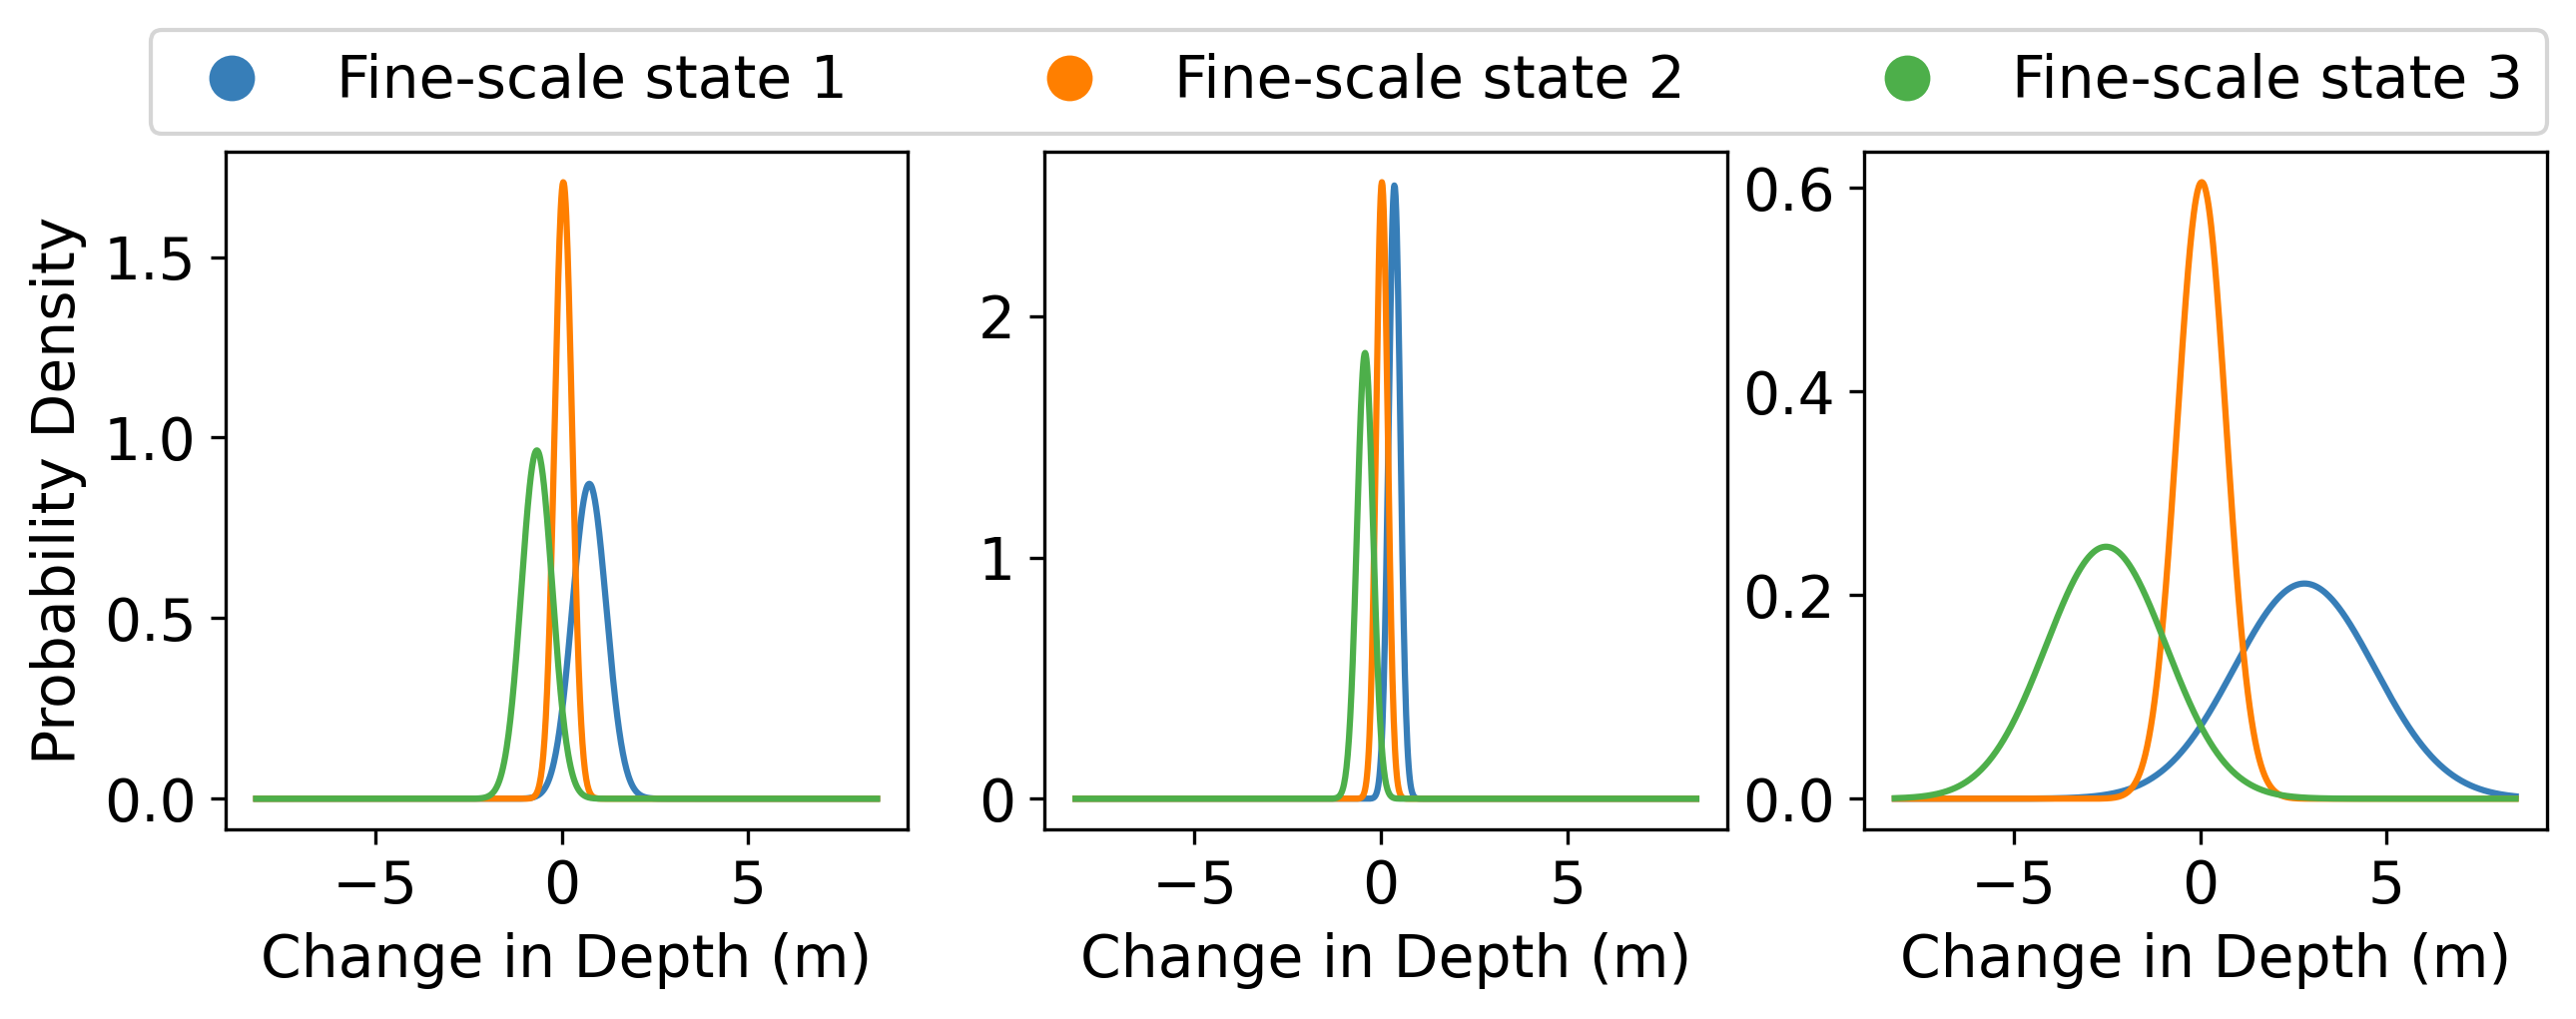
\includegraphics[width=6.5in]{../plt/emission_dists_K_3_3_nWhales_8.png}
    \caption{State-dependent density of change in depth for dive types 1, 2, and 3 (left to right). Fine-scale state 1 corresponds to descent, fine-scale state 2 corresponds to bottom, and fine-scale state 3 corresponds to ascent. Dive type 1 corresponds to medium-depth dives, dive type 2 corresponds to shallow dives, and dive type 3 corresponds to deep dives.}
    \label{fig:emission_dist}
\end{figure}

The coarse-scale, inter-dive transition probability matrix and initial distribution estimates were 

\begin{gather}
    \hat \bfGamma^{(c)} = 
    \begin{pmatrix} 
    0.223 & 0.758 & 0.017 \\
    0.123 & 0.853 & 0.027 \\
    0.074 & 0.857 & 0.068
    \end{pmatrix}, \\ \nonumber \\
    %
    \hat \bfdelta^{(c)} = \begin{pmatrix} 0.258 & 0.002 & 0.740 \end{pmatrix}.
\end{gather}

The long-run proportion of each dive type is found by solving for the stationary distribution of $\hat \bfGamma^{(c)}$, i.e. solving the equation $\hat \bfpi^{(c)} \hat \bfGamma^{(c)} = \hat \bfpi^{(c)}$. Doing so gives the following:
%
\begin{equation}
    \hat \bfpi^{(c)} = 
    \begin{pmatrix}
        0.136 & 0.840 & 0.024
    \end{pmatrix}.
\end{equation}
%
In words, approximately 13.6\% of all dives are of type 1 (medium-depth), 84.0\% of all dives are of type 2 (shallow), and 2.4\% of all dives are of type 3 (deep).

The fine-scale, intra-dive transition probability matrices and initial distributions were estimated as

\begin{gather}
    \hat \bfGamma^{(f,1)} = 
    \begin{pmatrix} 
    0.871 & 0.123 & 0.006 \\
    \bf{0} & 0.962 & 0.038 \\
    \bf{0} & \bf{0} & \bf{1}
    \end{pmatrix}, \quad
    %
    \hat \bfGamma^{(f,2)} = 
    \begin{pmatrix} 
    0.668 & 0.304 & 0.028 \\
    \bf{0} & 0.788 & 0.212 \\
    \bf{0} & \bf{0} & \bf{1}
    \end{pmatrix}, ~
    \\ \nonumber \\
    \hat \bfGamma^{(f,3)} = 
    \begin{pmatrix} 
    0.958 & 0.040 & 0.002 \\
    \bf{0} & 0.982 & 0.018 \\
    \bf{0} & \bf{0} & \bf{1}
    \end{pmatrix}, \\ \nonumber \\
    %
    \hat \bfdelta^{(f,1)} = \begin{pmatrix} \bf{1} & \bf{0} & \bf{0} \end{pmatrix}, \quad ~
    %
    \hat \bfdelta^{(f,2)} = \begin{pmatrix} \bf{1} & \bf{0} & \bf{0} \end{pmatrix}, \quad ~
    %
    \hat \bfdelta^{(f,3)} = \begin{pmatrix} \bf{1} & \bf{0} & \bf{0} \end{pmatrix}
\end{gather}

Recall that each dive must begin with descent, so all initial distributions are identical. In addition, note that the Markov chains defined by $\hat \bfGamma^{(f,i)}$ above are not ergodic, so stationary distributions do not exist for the fine-scale, intra-dive Markov chains.

\section{Case study decoded dive profiles}

The figures below show approximately one hour of dive profiles associated with each of the eight whales used to train the hierarchical HMM in the case study.

\begin{figure}[H]
    \centering
    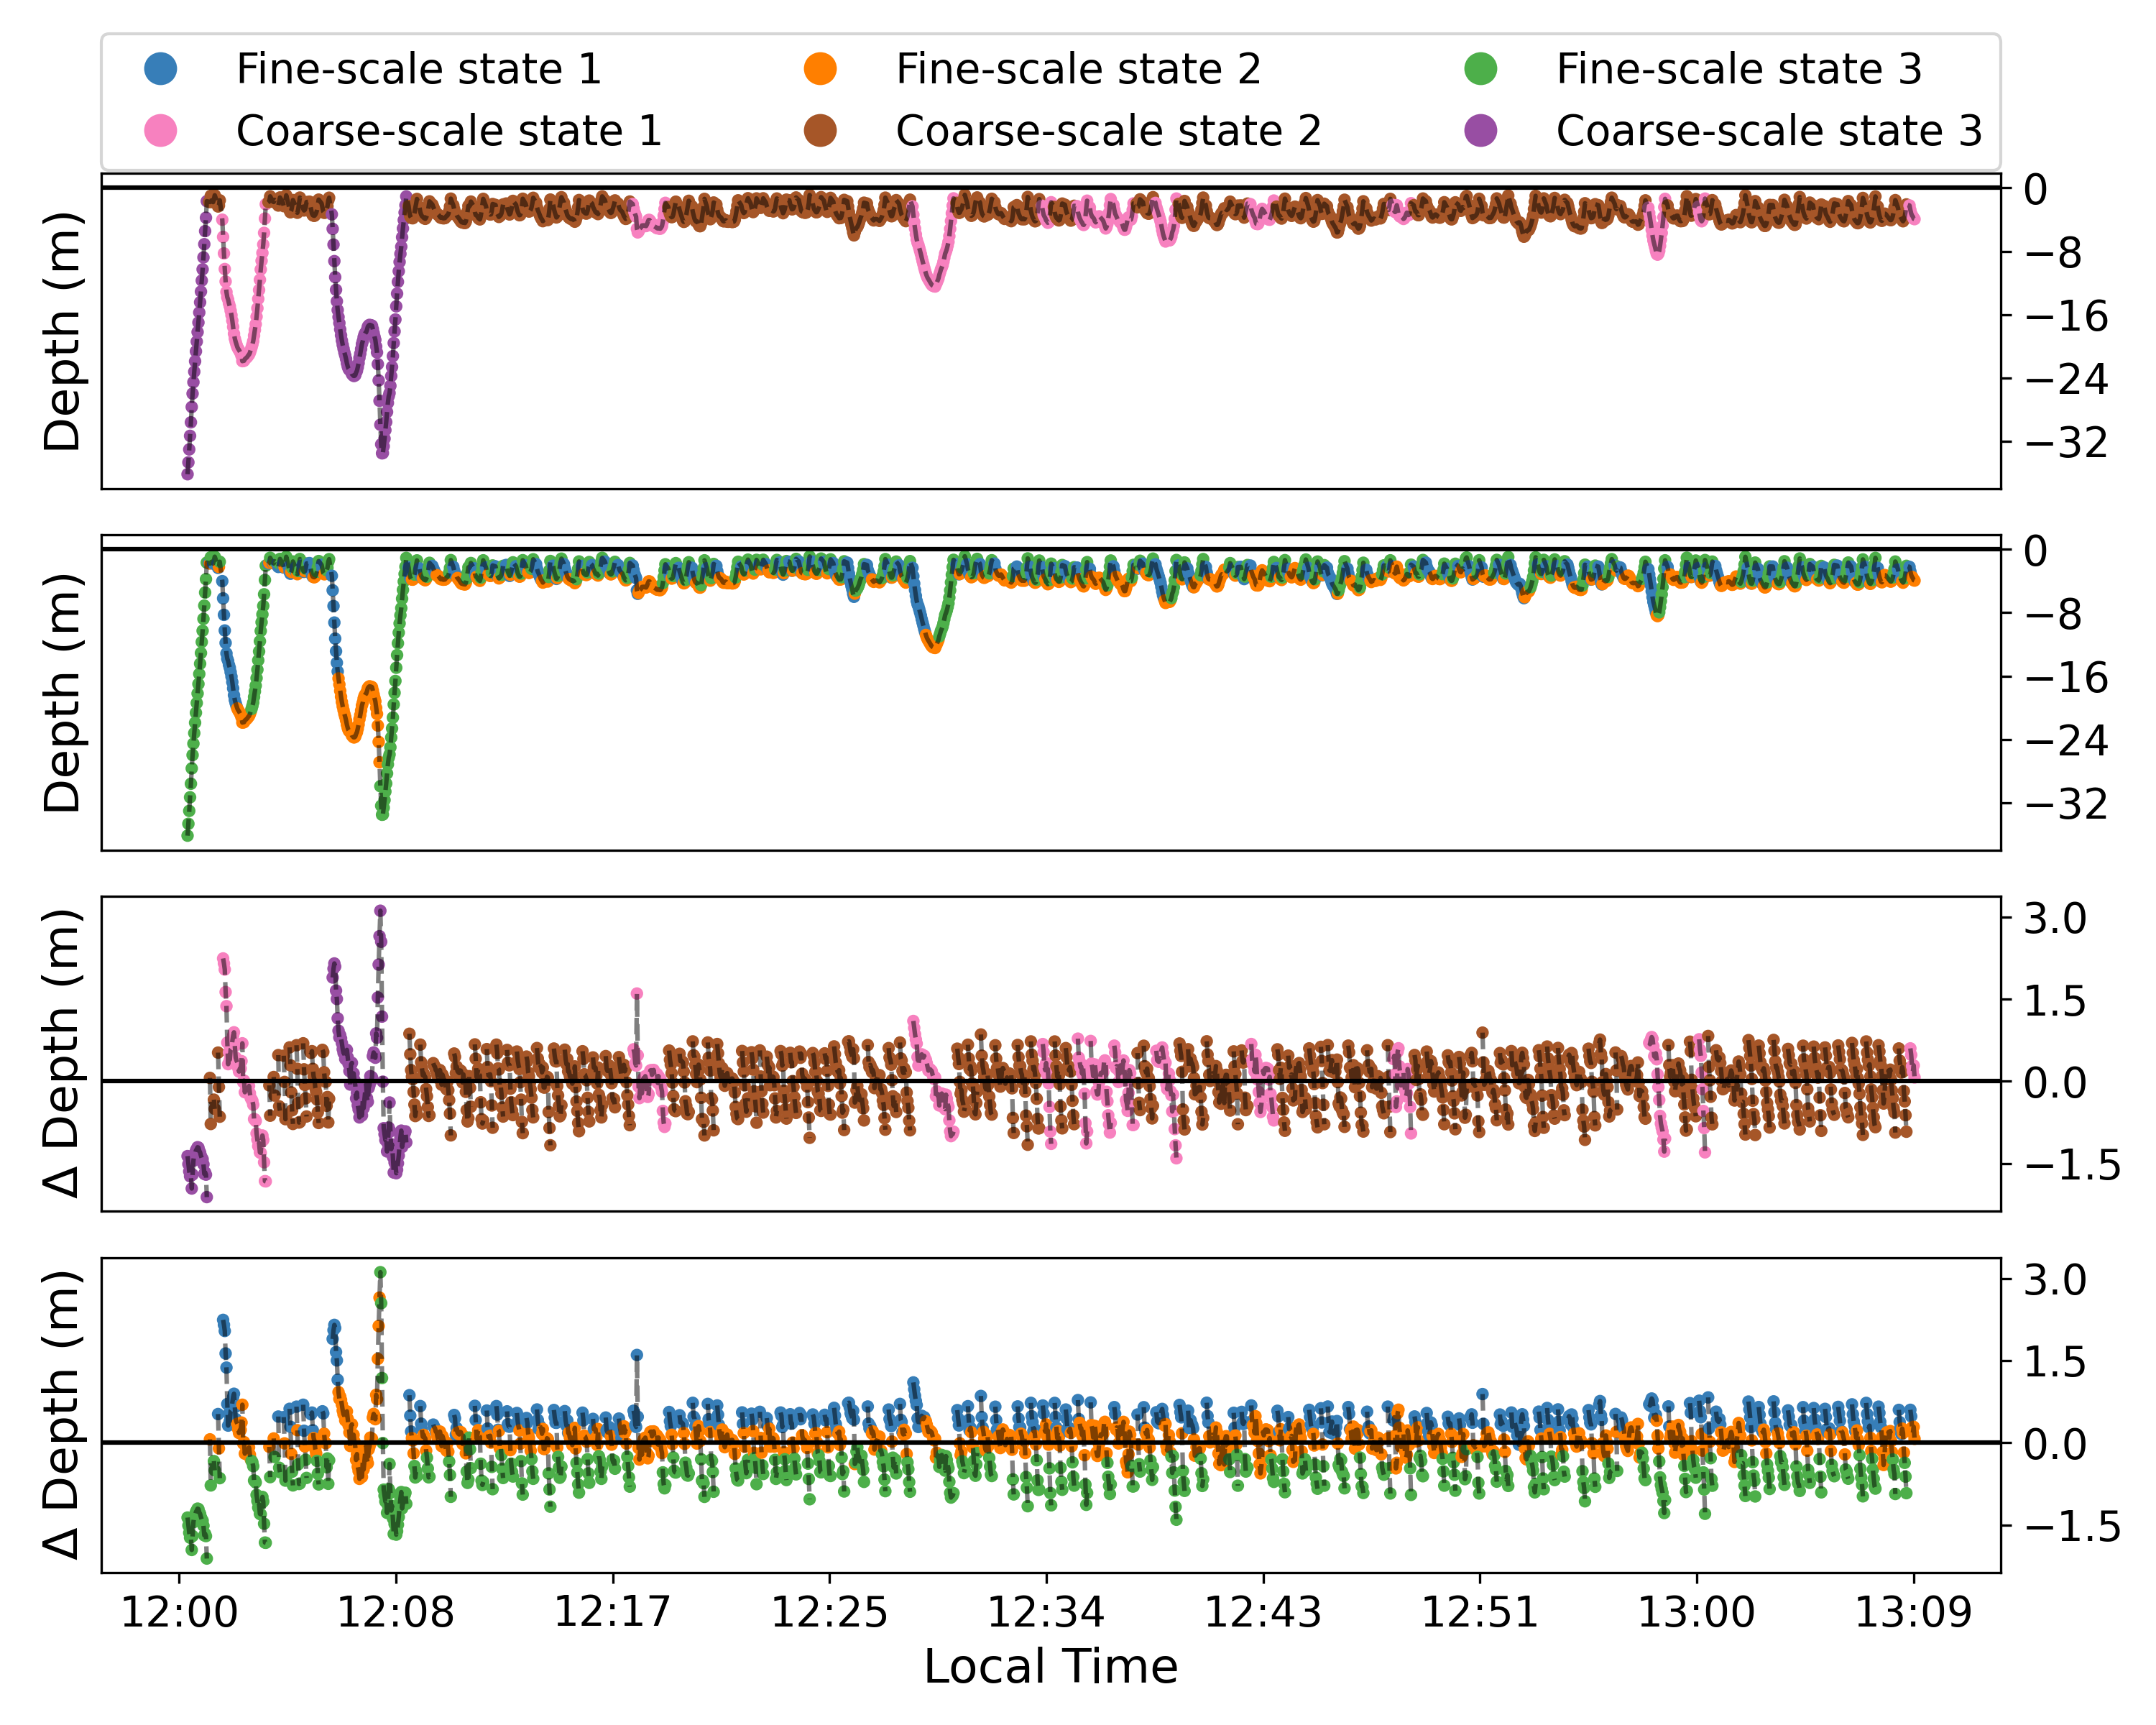
\includegraphics[width=6.5in]{../plt/decoded_dives_kw_A100_K_3_3_nWhales_8.png}
    \caption{Dive profiles and change in depth vs time for a selected hour of dive time for killer whale A100. All data is color-coded by most likely dive type (rows one and three) as well as most likely dive phase (rows two and four).}
    \label{fig:A100}
\end{figure}

\begin{figure}[H]
    \centering
    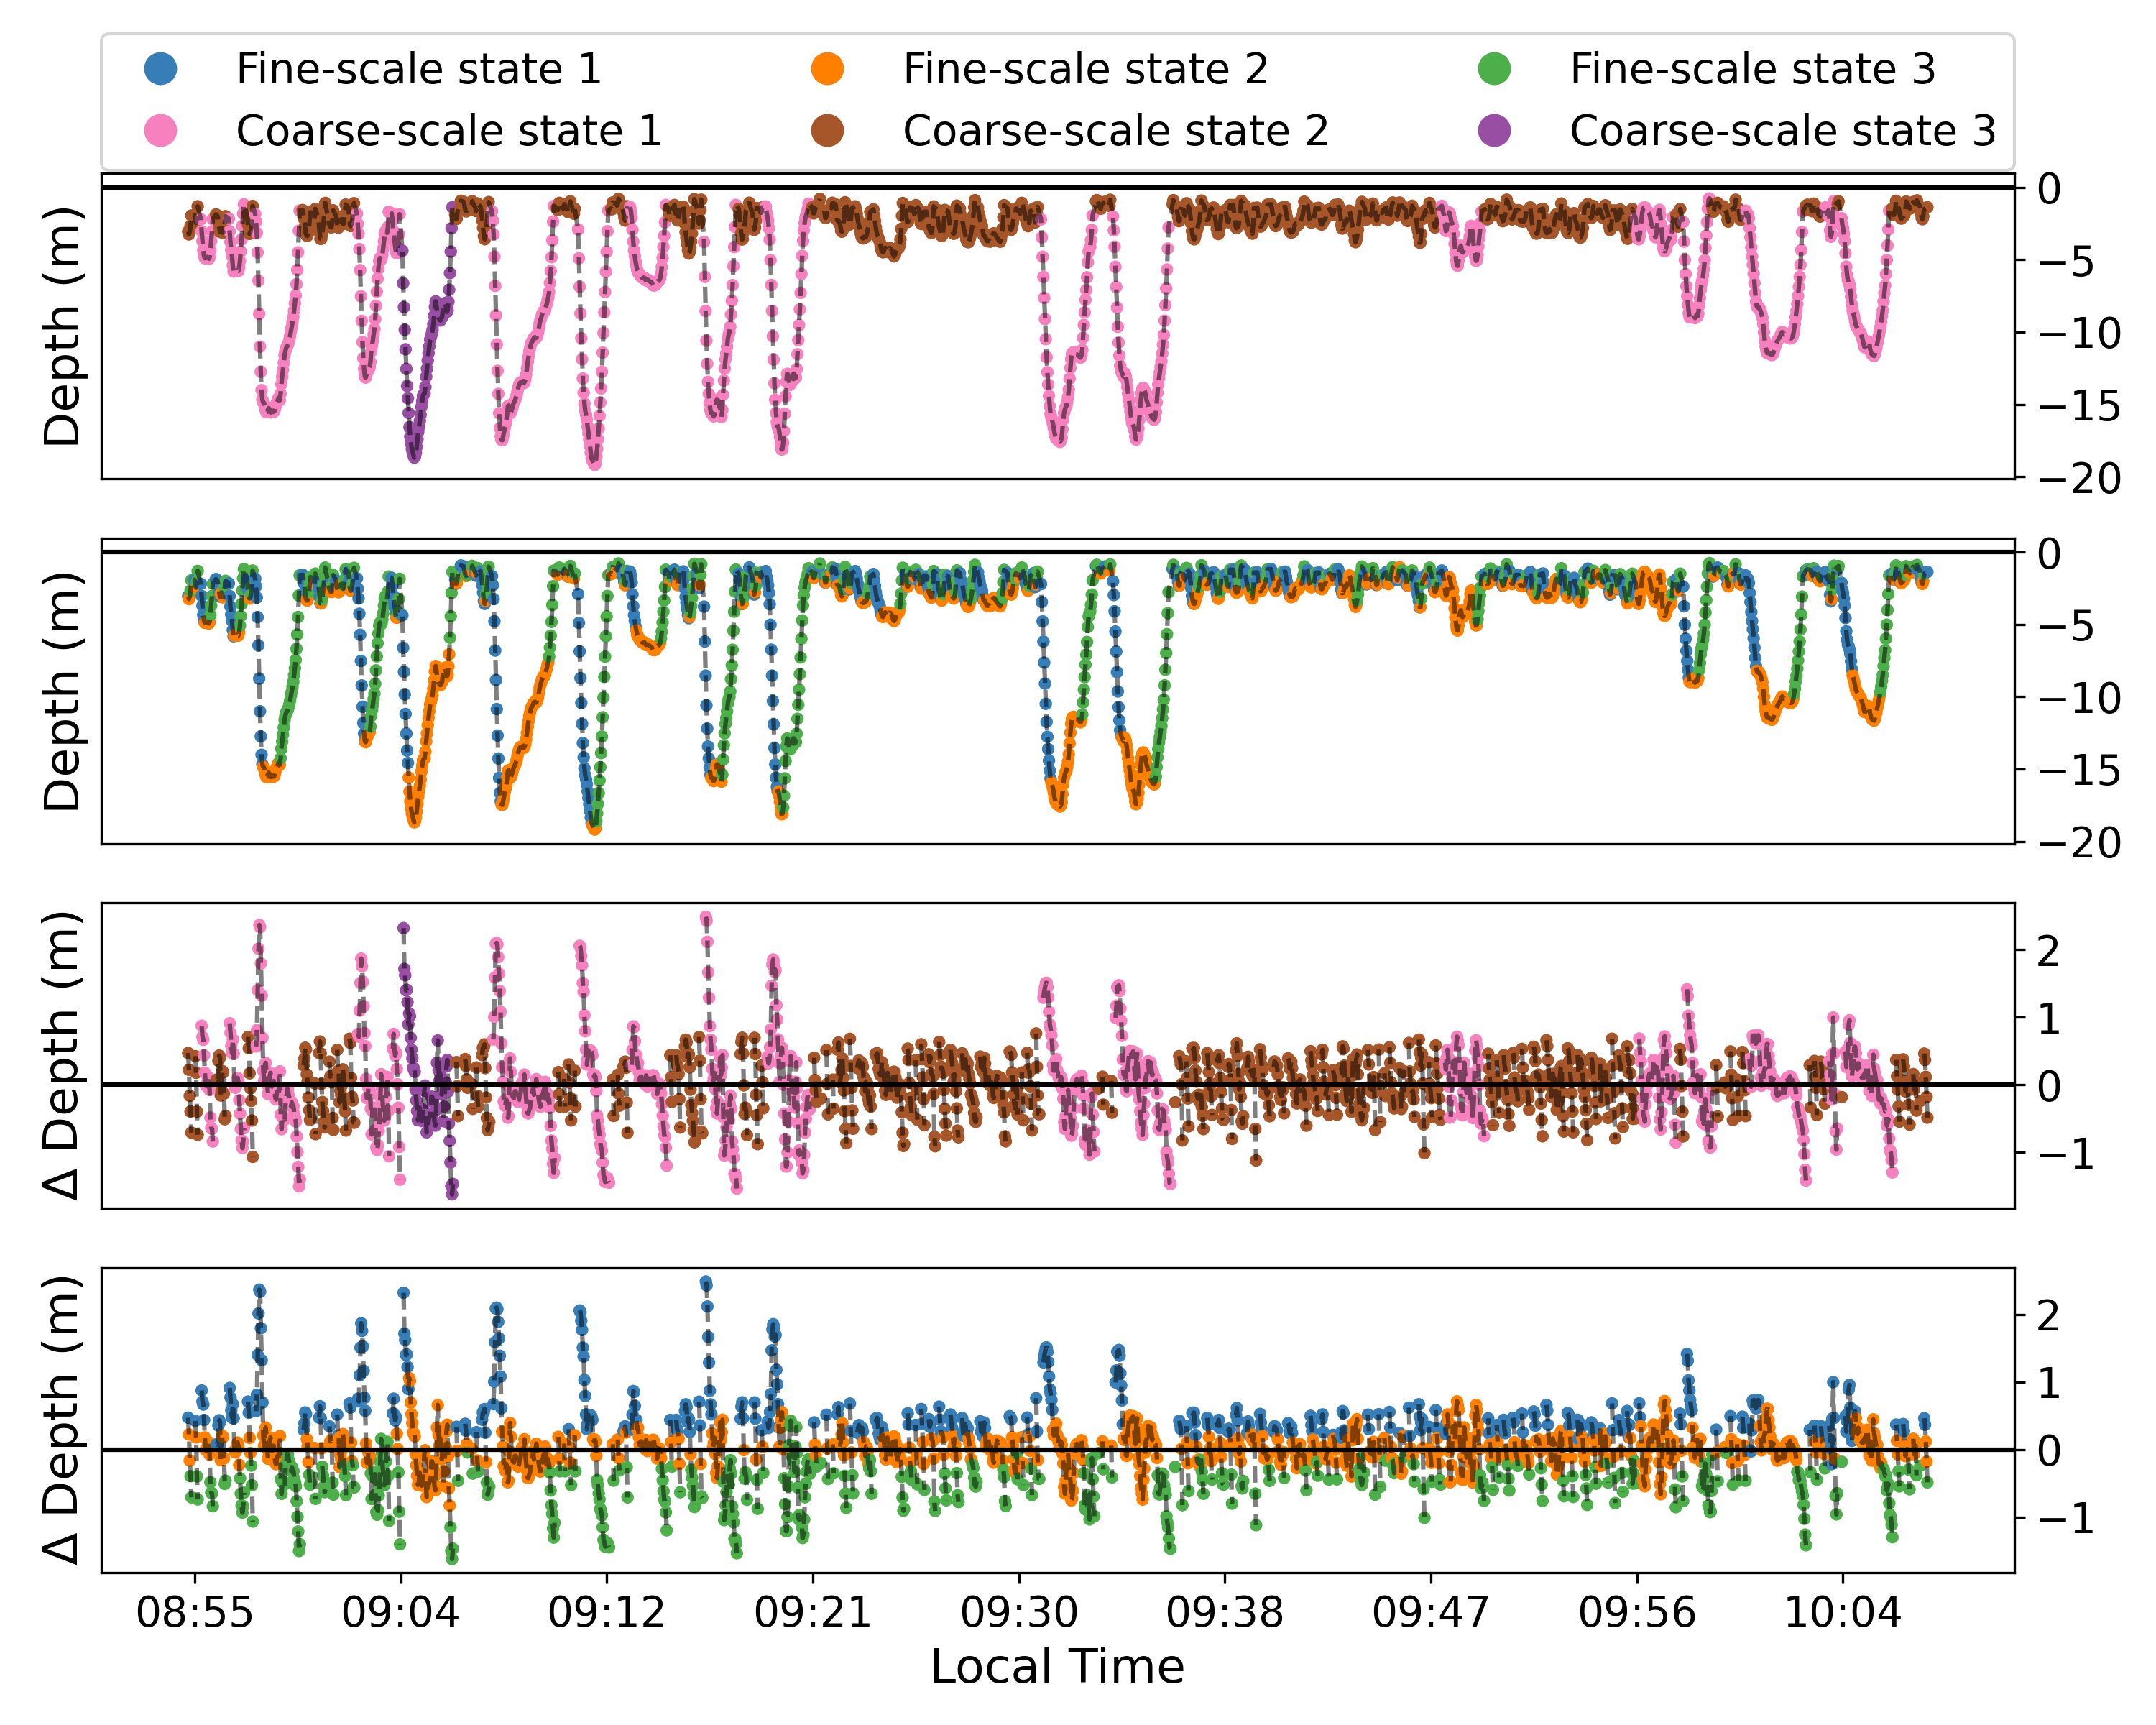
\includegraphics[width=6.5in]{../plt/decoded_dives_kw_A113_K_3_3_nWhales_8.png}
    \caption{Dive profiles and change in depth vs time for a selected hour of dive time for killer whale A113. All data is color-coded by most likely dive type (rows one and three) as well as most likely dive phase (rows two and four).}
    \label{fig:A113}
\end{figure}

\begin{figure}[H]
    \centering
    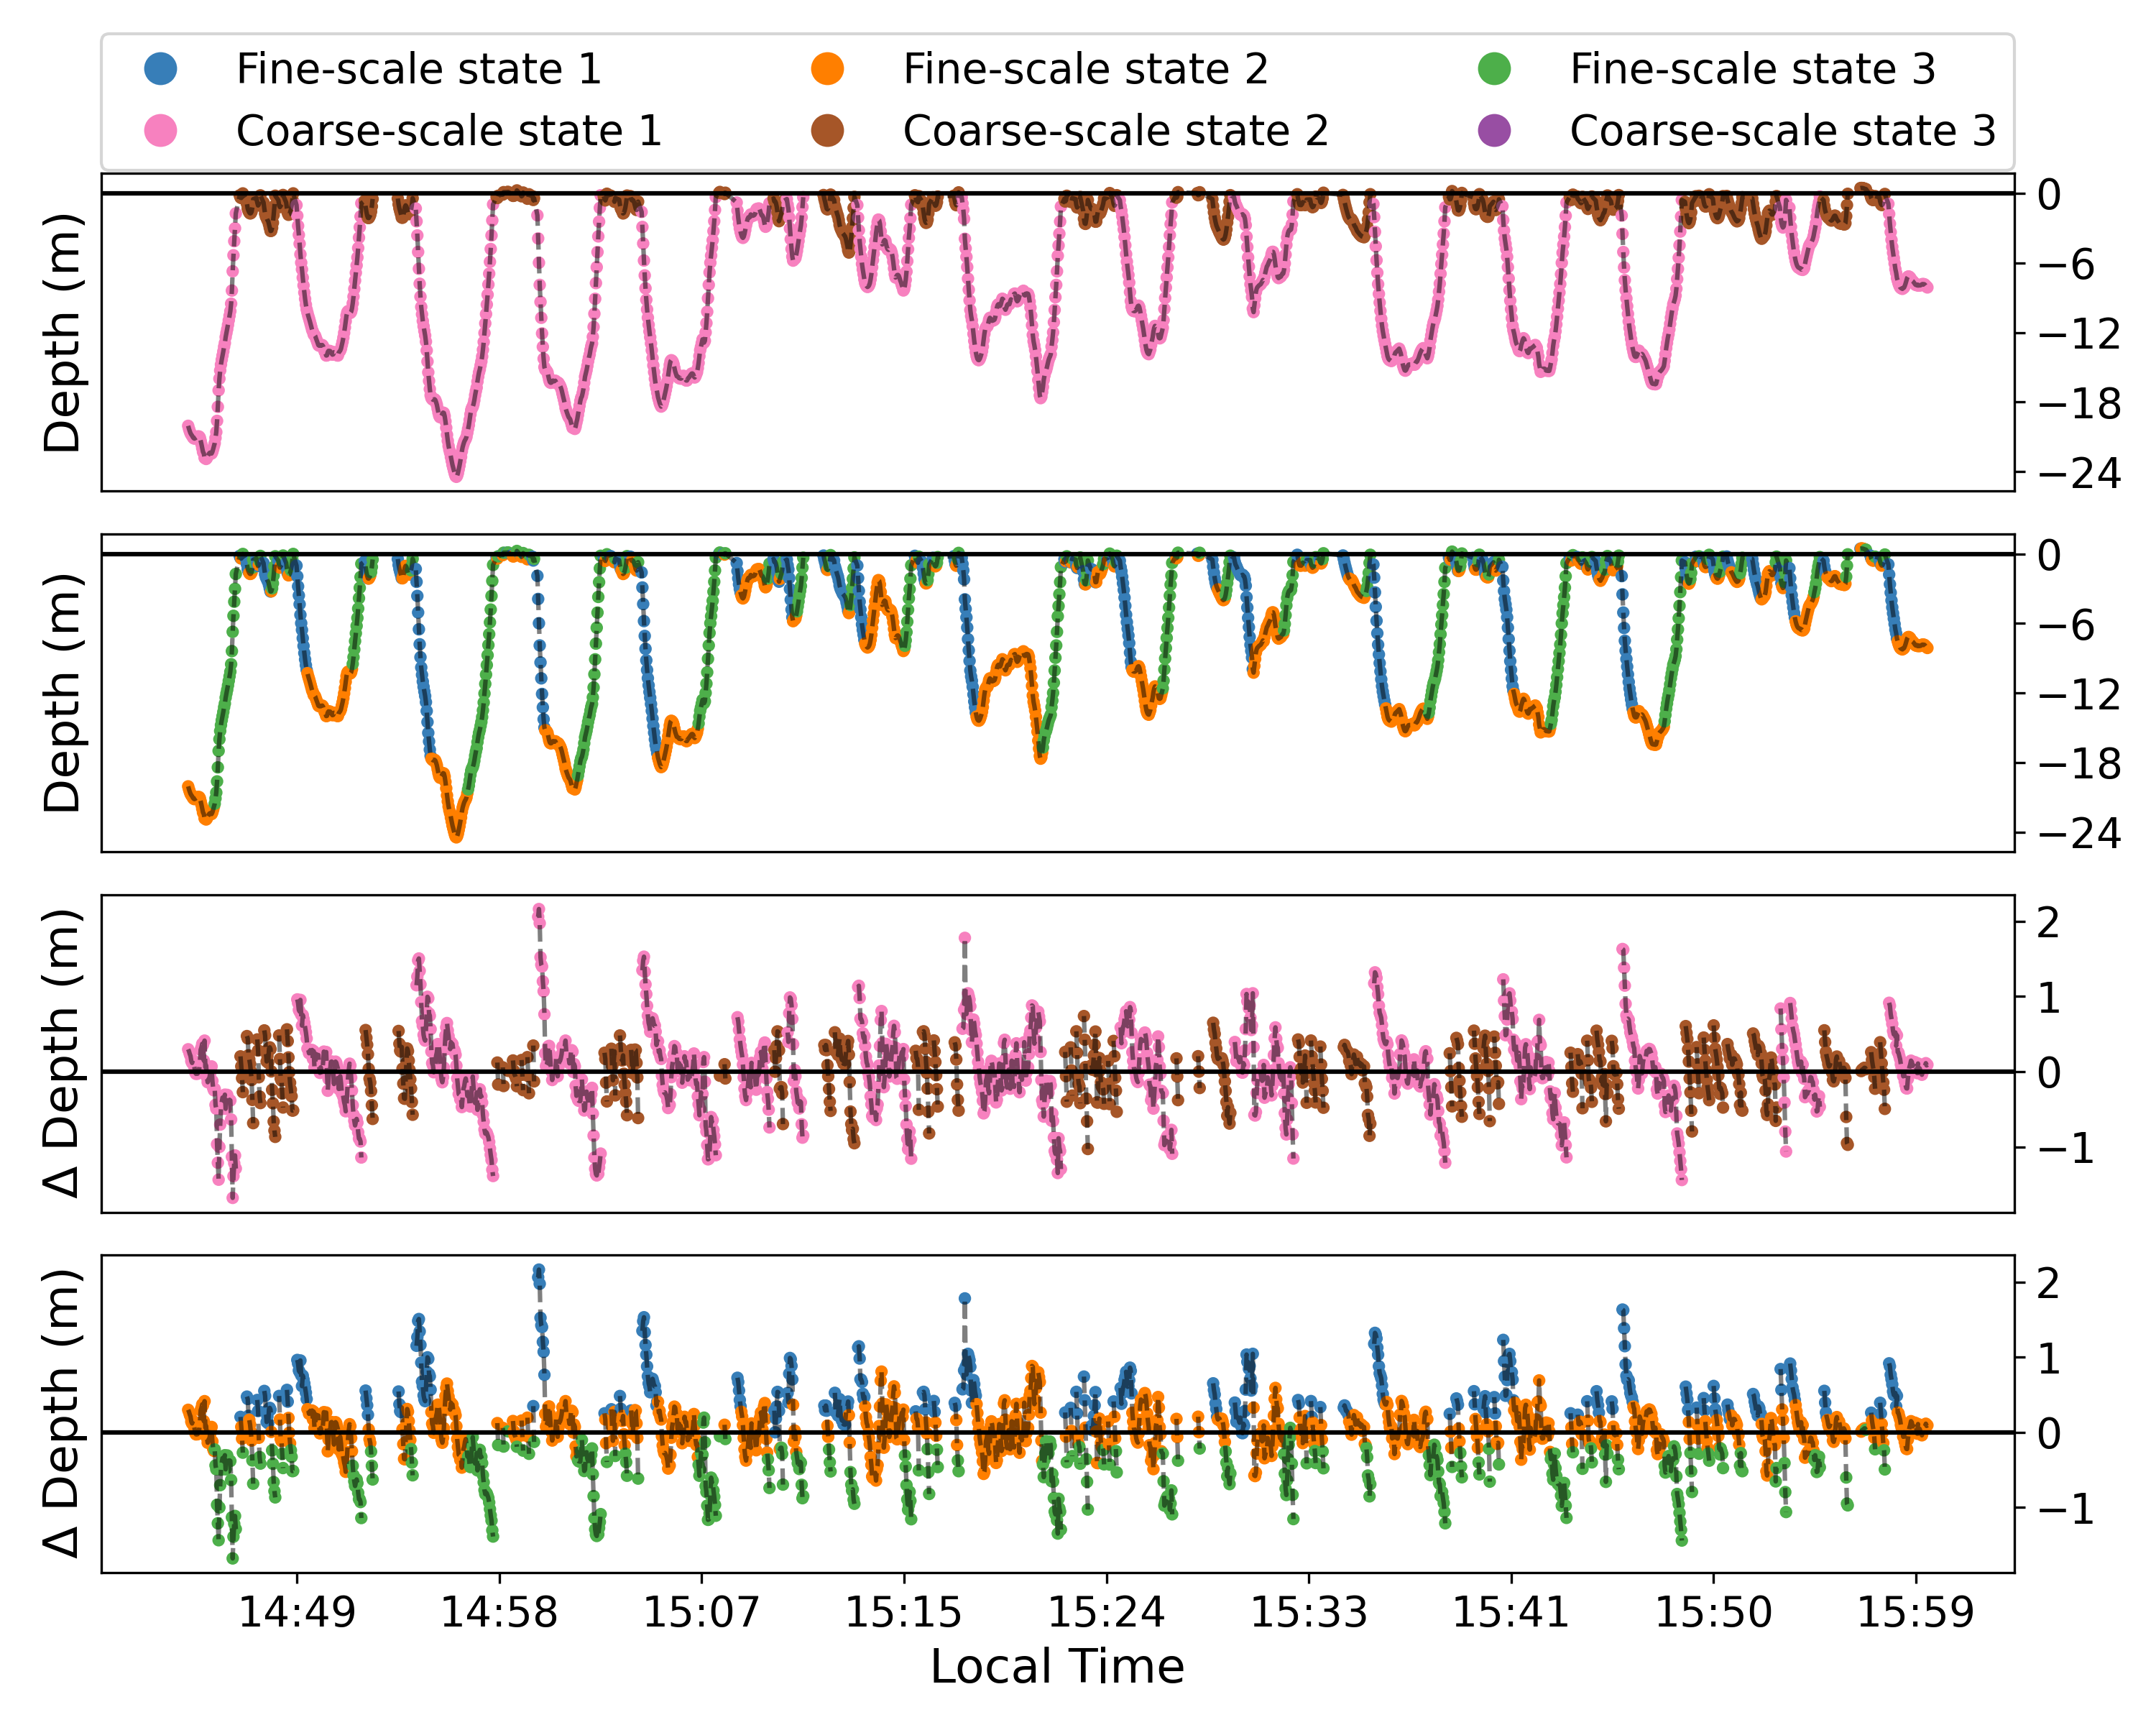
\includegraphics[width=6.5in]{../plt/decoded_dives_kw_D21_K_3_3_nWhales_8.png}
    \caption{Dive profiles and change in depth vs time for a selected hour of dive time for killer whale D21. All data is color-coded by most likely dive type (rows one and three) as well as most likely dive phase (rows two and four).}
    \label{fig:D21}
\end{figure}

\begin{figure}[H]
    \centering
    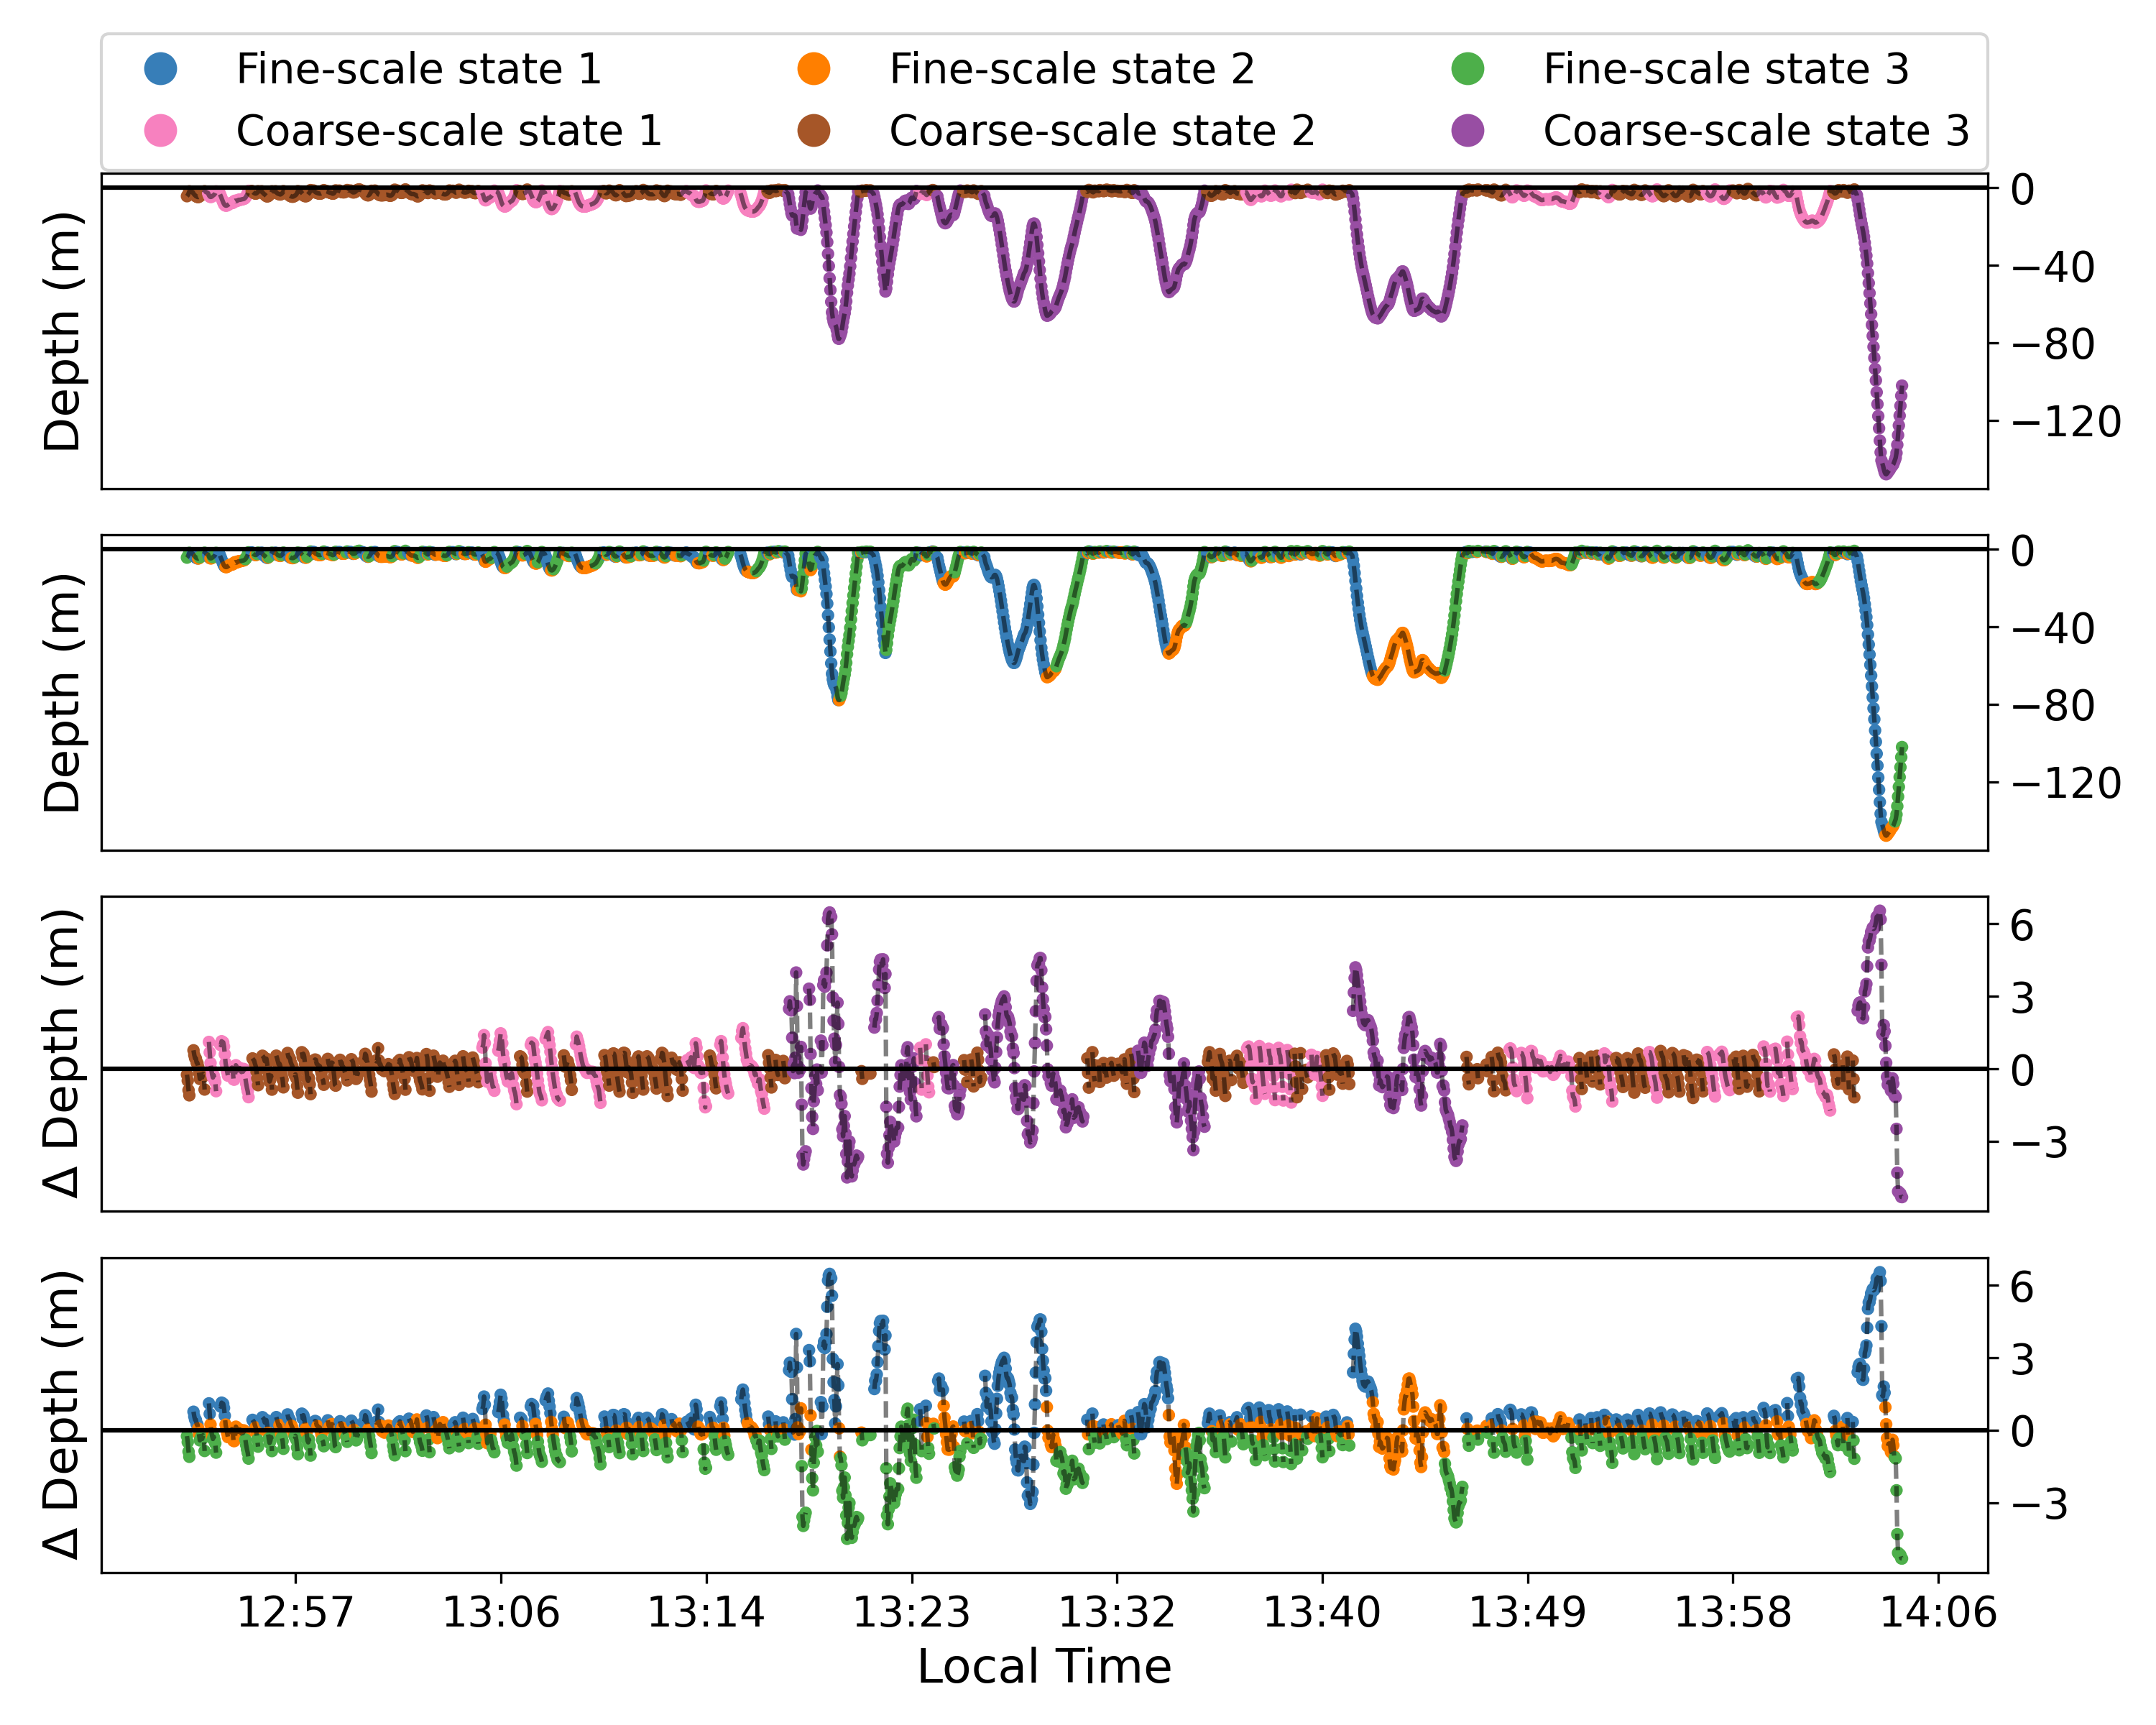
\includegraphics[width=6.5in]{../plt/decoded_dives_kw_D26_K_3_3_nWhales_8.png}
    \caption{Dive profiles and change in depth vs time for a selected hour of dive time for killer whale D26. All data is color-coded by most likely dive type (rows one and three) as well as most likely dive phase (rows two and four).}
    \label{fig:D26}
\end{figure}

\begin{figure}[H]
    \centering
    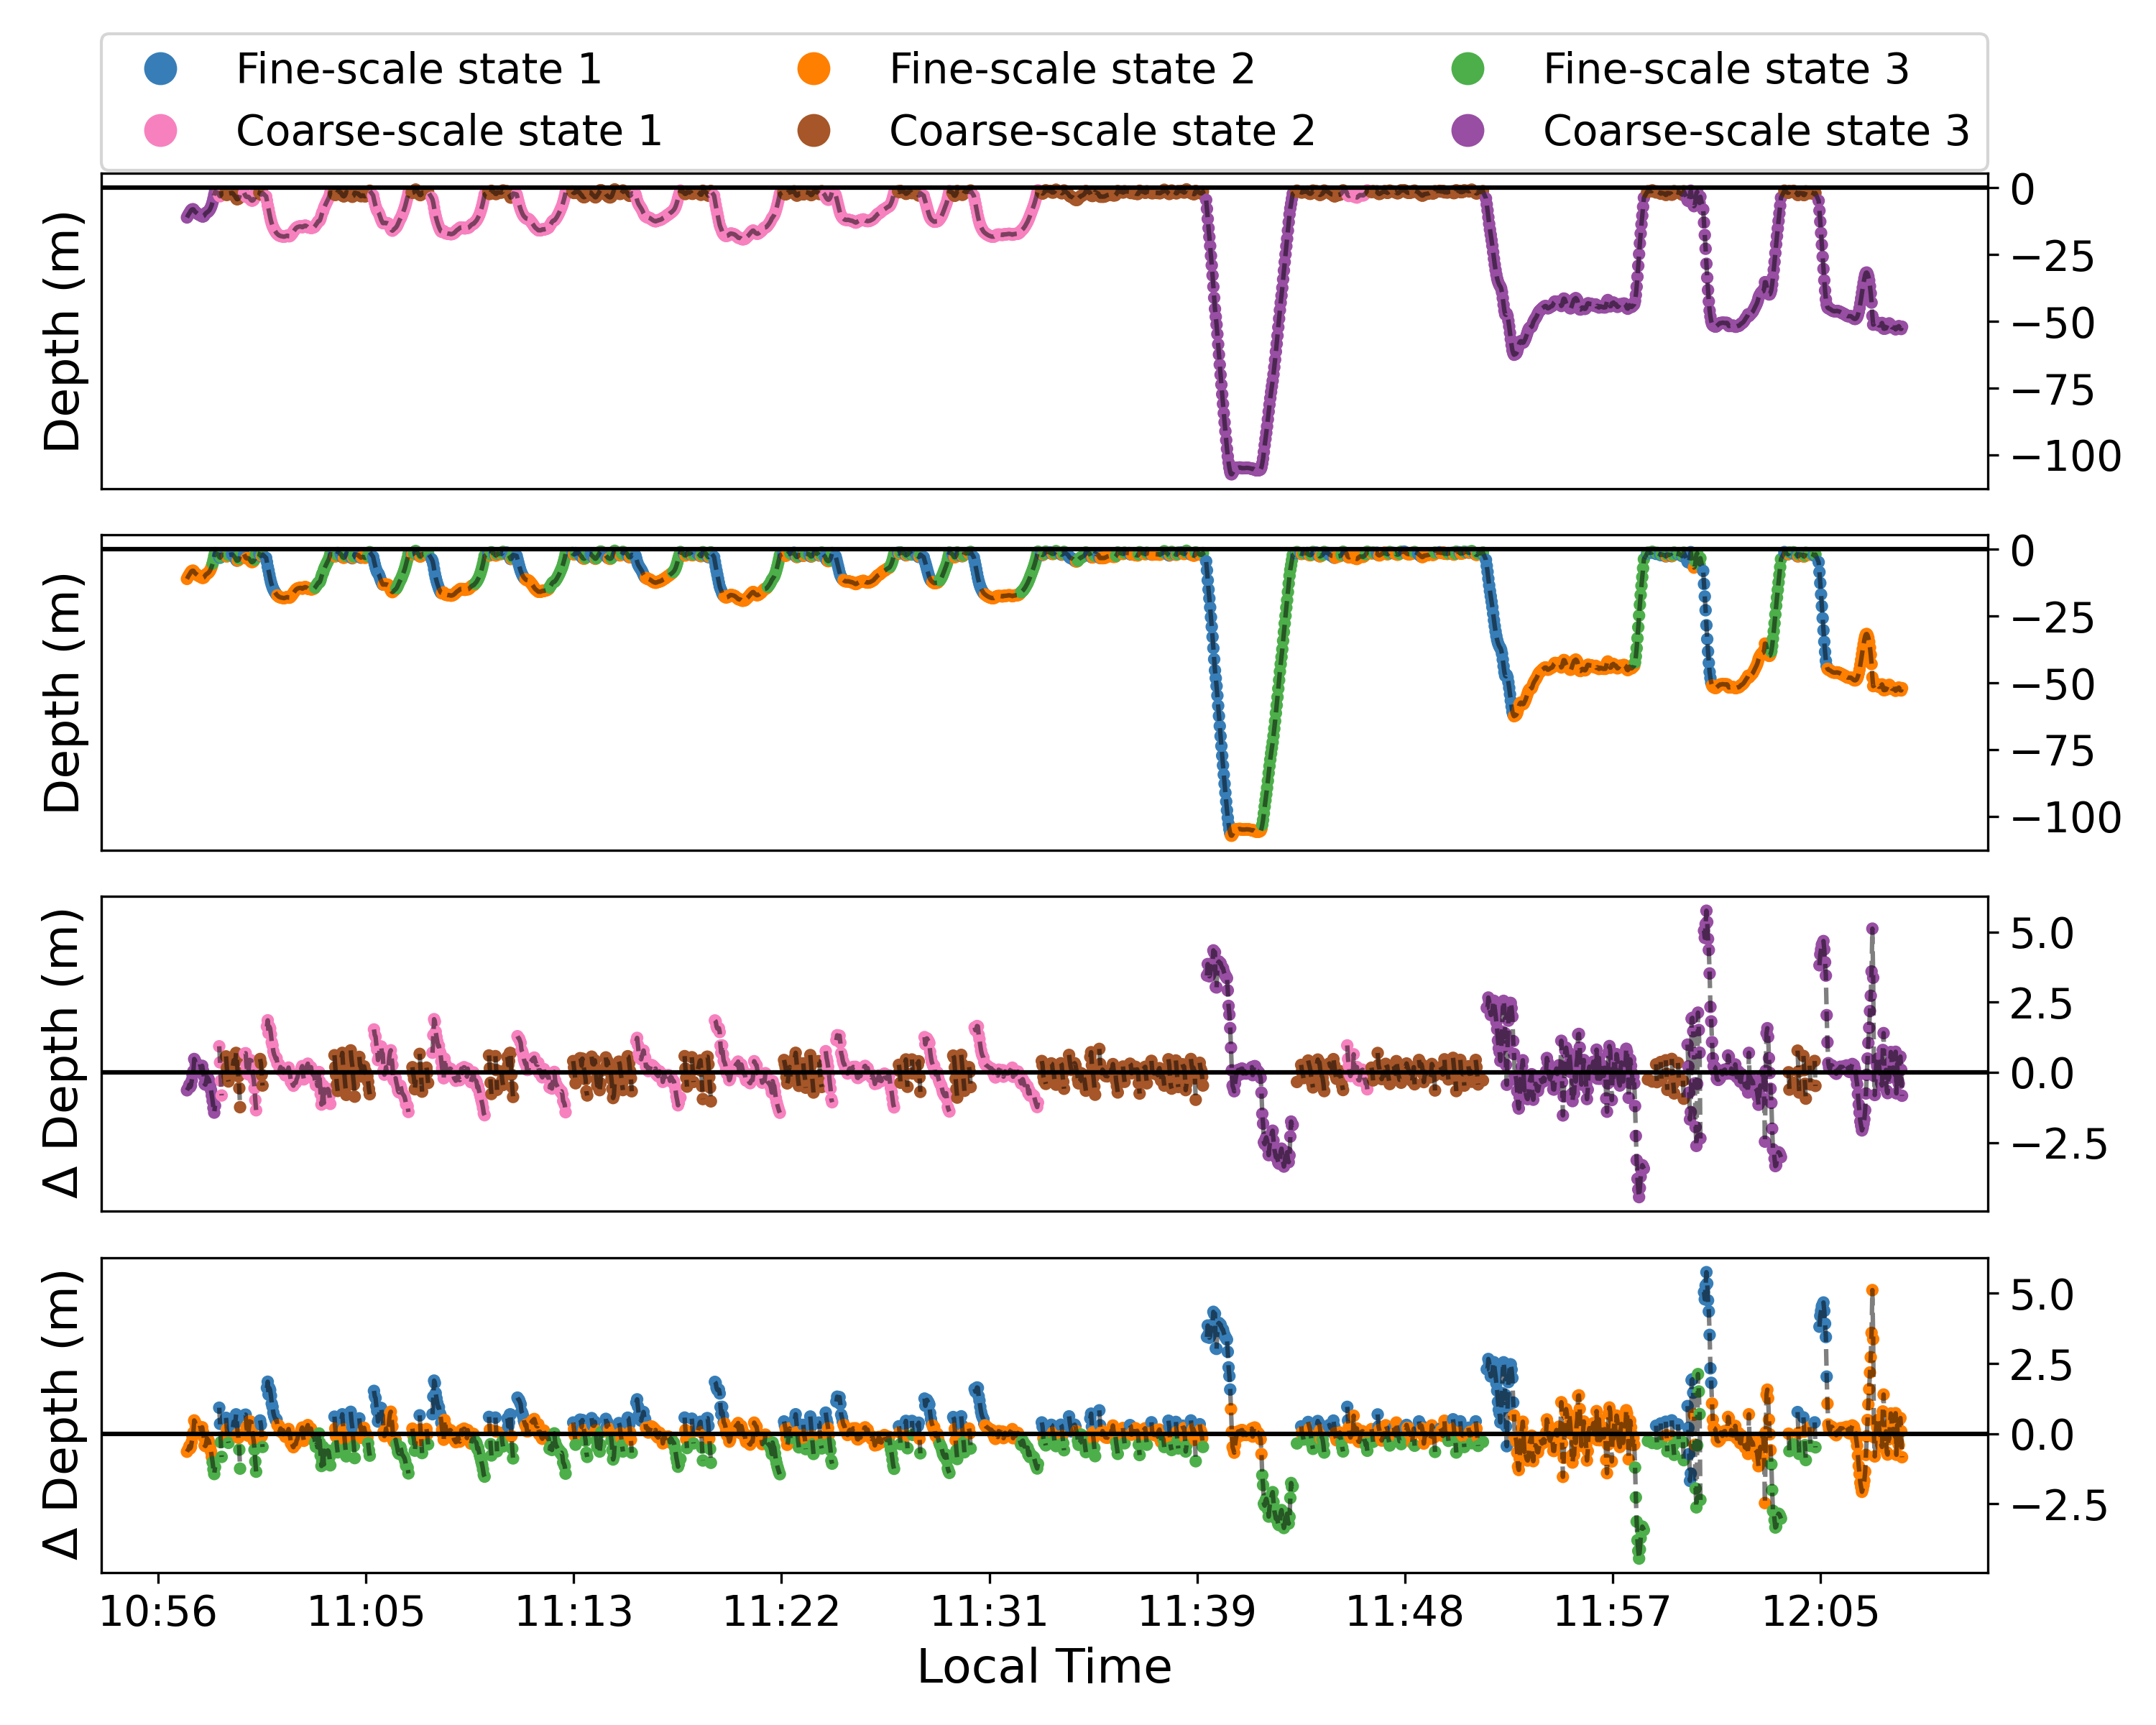
\includegraphics[width=6.5in]{../plt/decoded_dives_kw_I107_K_3_3_nWhales_8.png}
    \caption{Dive profiles and change in depth vs time for a selected hour of dive time for killer whale I107. All data is color-coded by most likely dive type (rows one and three) as well as most likely dive phase (rows two and four).}
    \label{fig:I107}
\end{figure}

\begin{figure}[H]
    \centering
    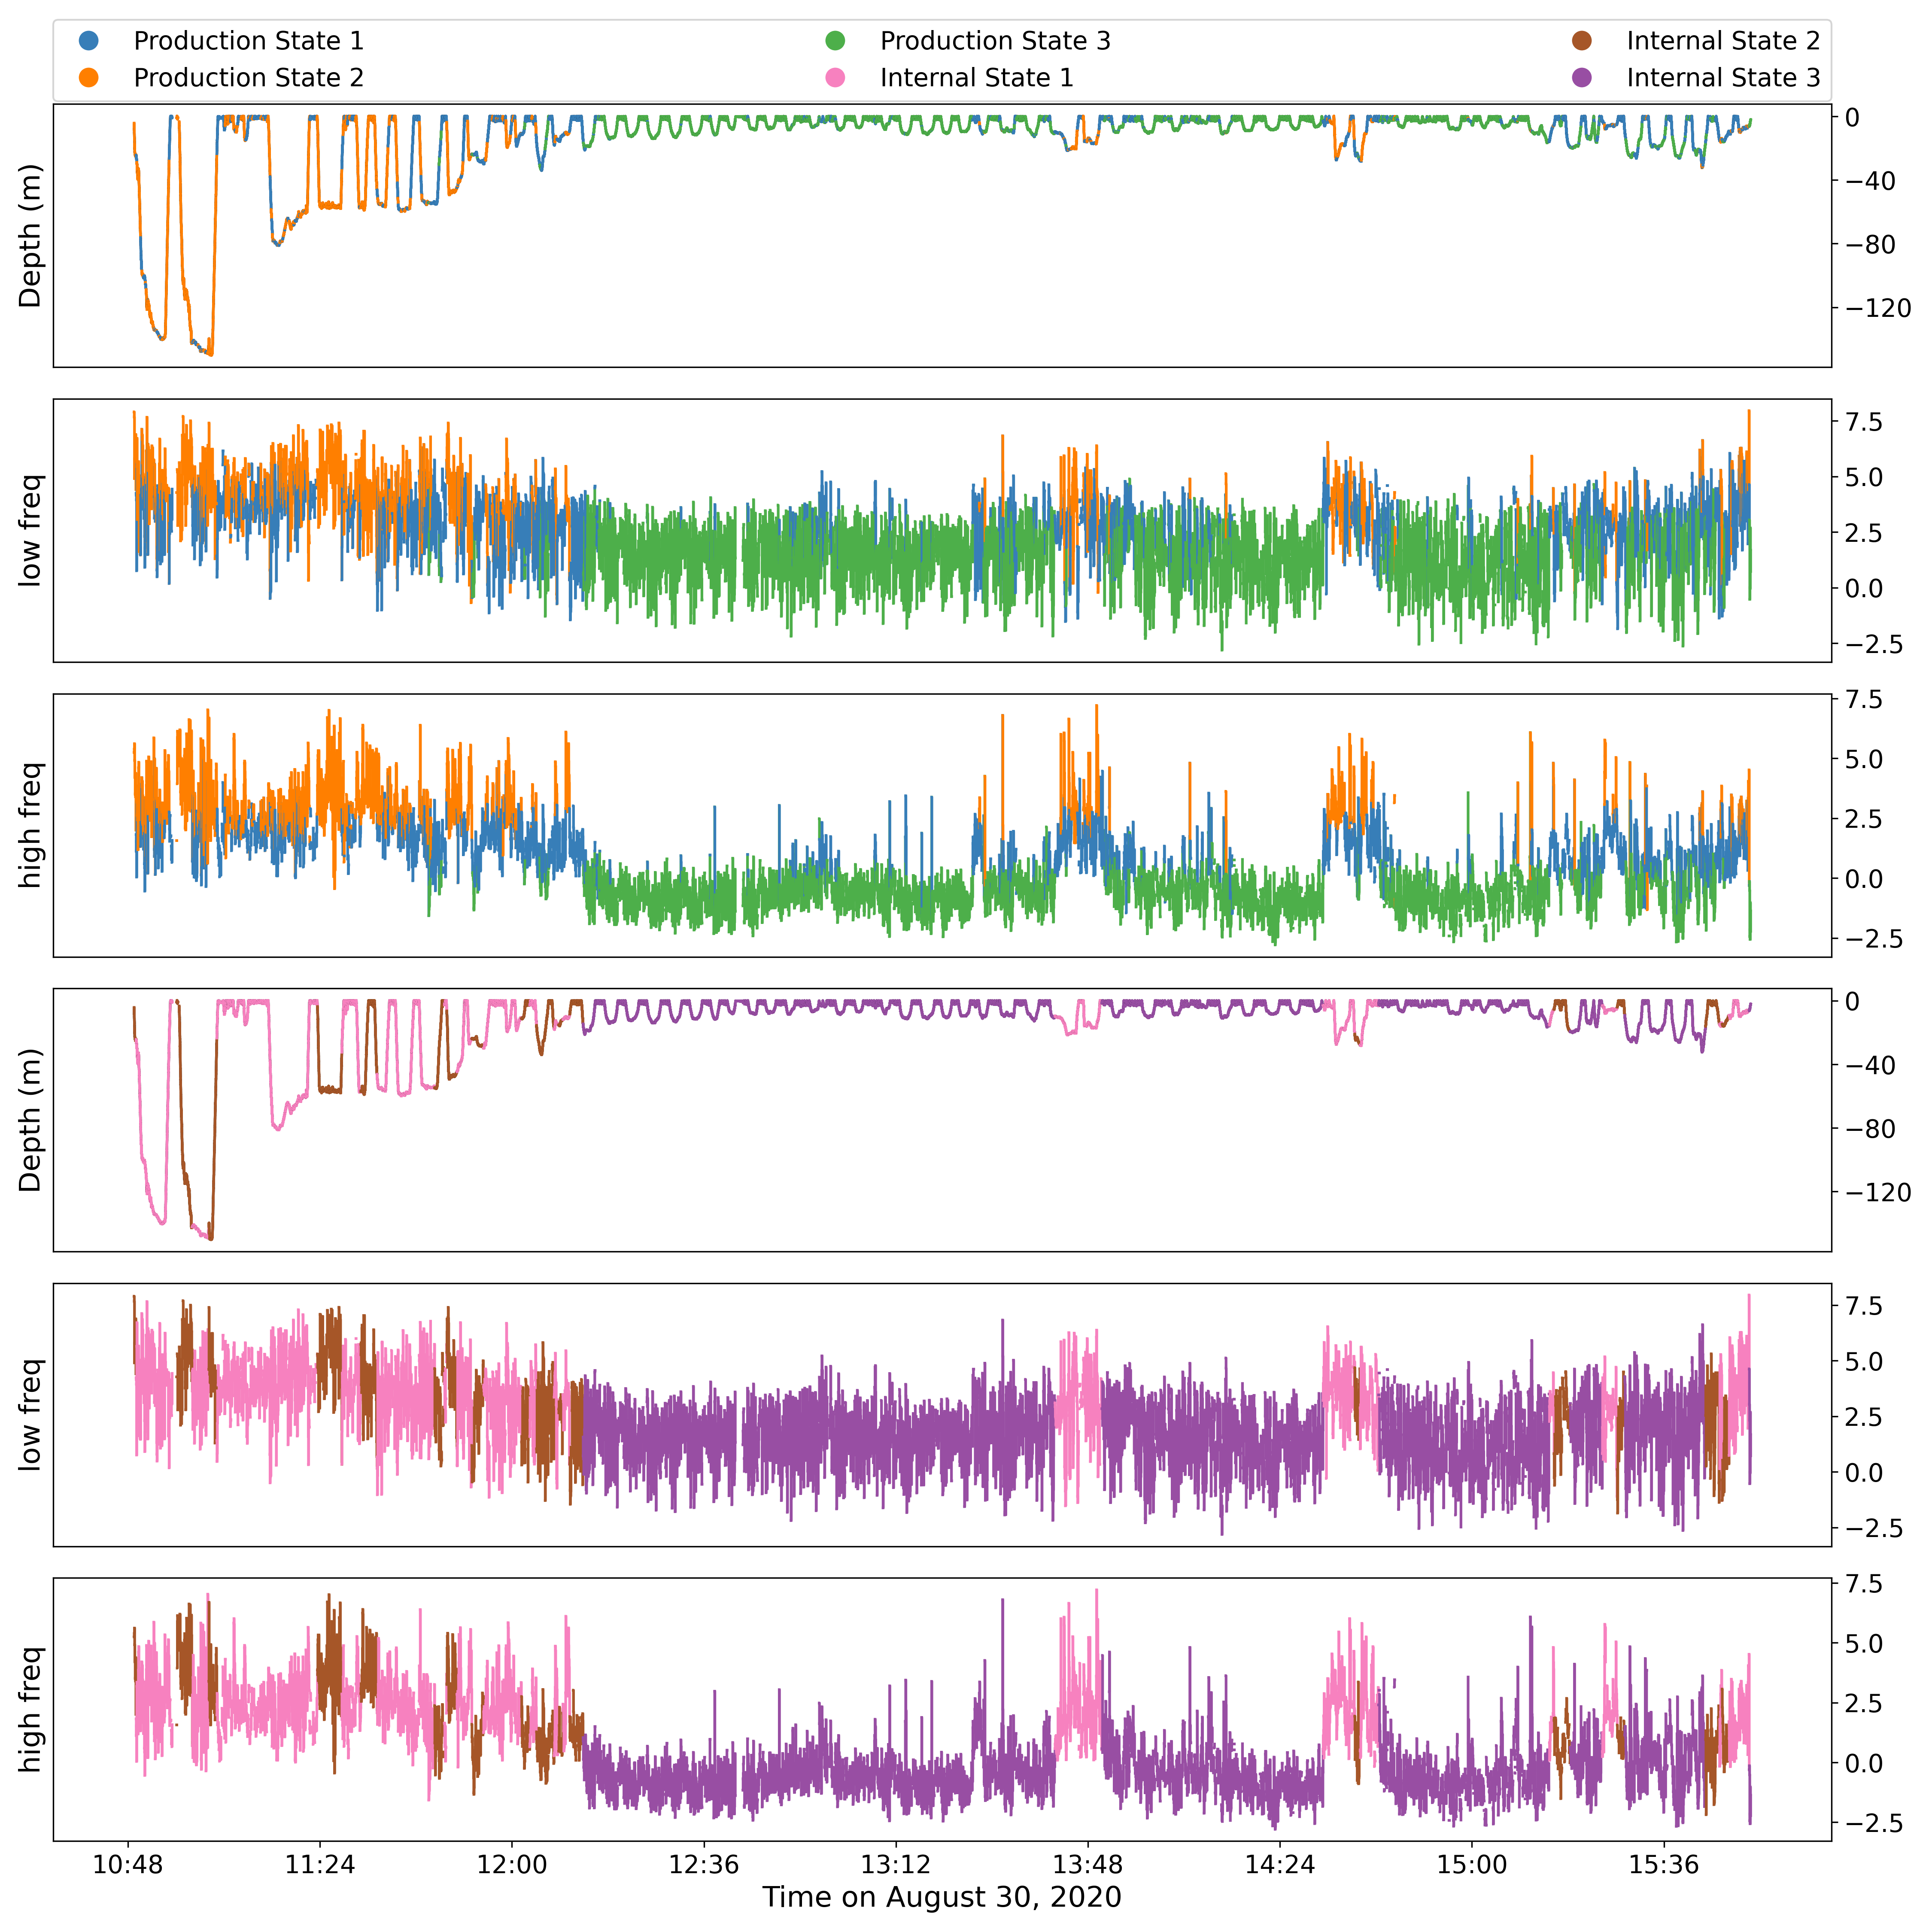
\includegraphics[width=6.5in]{../plt/decoded_dives_kw_I145_K_3_3_nWhales_8.png}
    \caption{Dive profiles and change in depth vs time for a selected hour of dive time for killer whale I145. All data is color-coded by most likely dive type (rows one and three) as well as most likely dive phase (rows two and four).}
    \label{fig:I145}
\end{figure}

\begin{figure}[H]
    \centering
    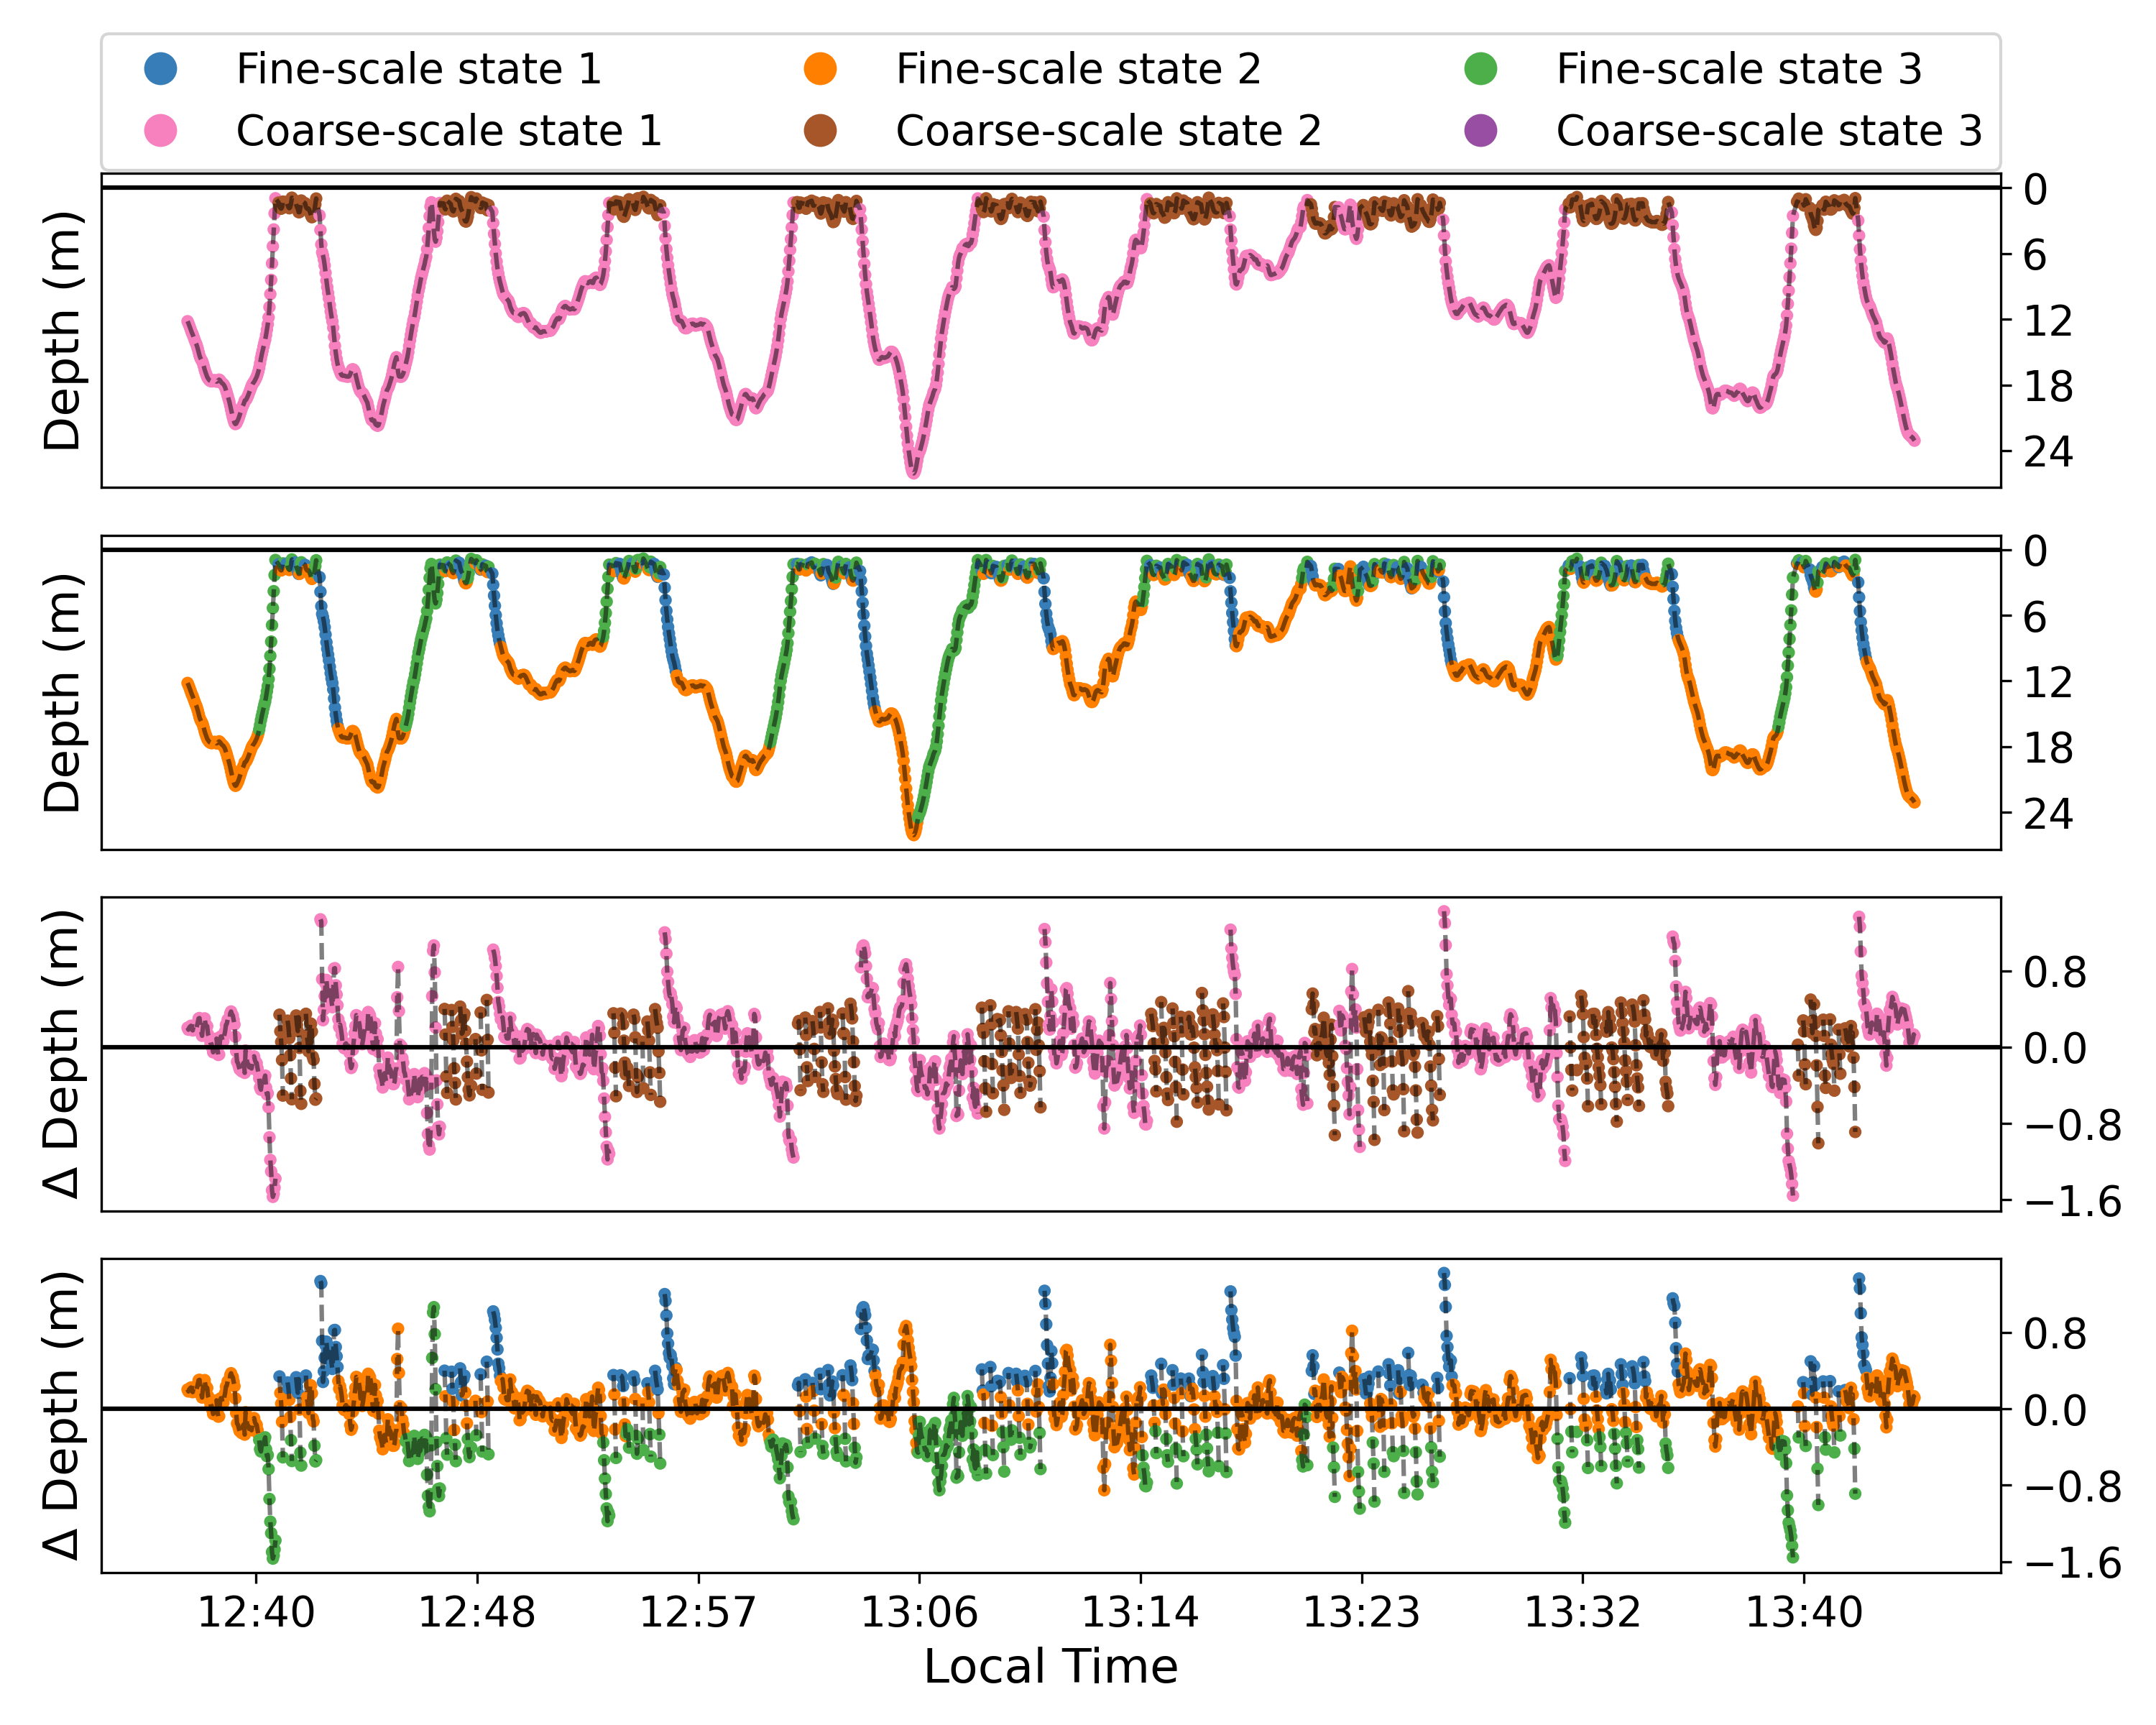
\includegraphics[width=6.5in]{../plt/decoded_dives_kw_R48_K_3_3_nWhales_8.png}
    \caption{Dive profiles and change in depth vs time for a selected hour of dive time for killer whale R48. All data is color-coded by most likely dive type (rows one and three) as well as most likely dive phase (rows two and four).}
    \label{fig:R48}
\end{figure}

\begin{figure}[H]
    \centering
    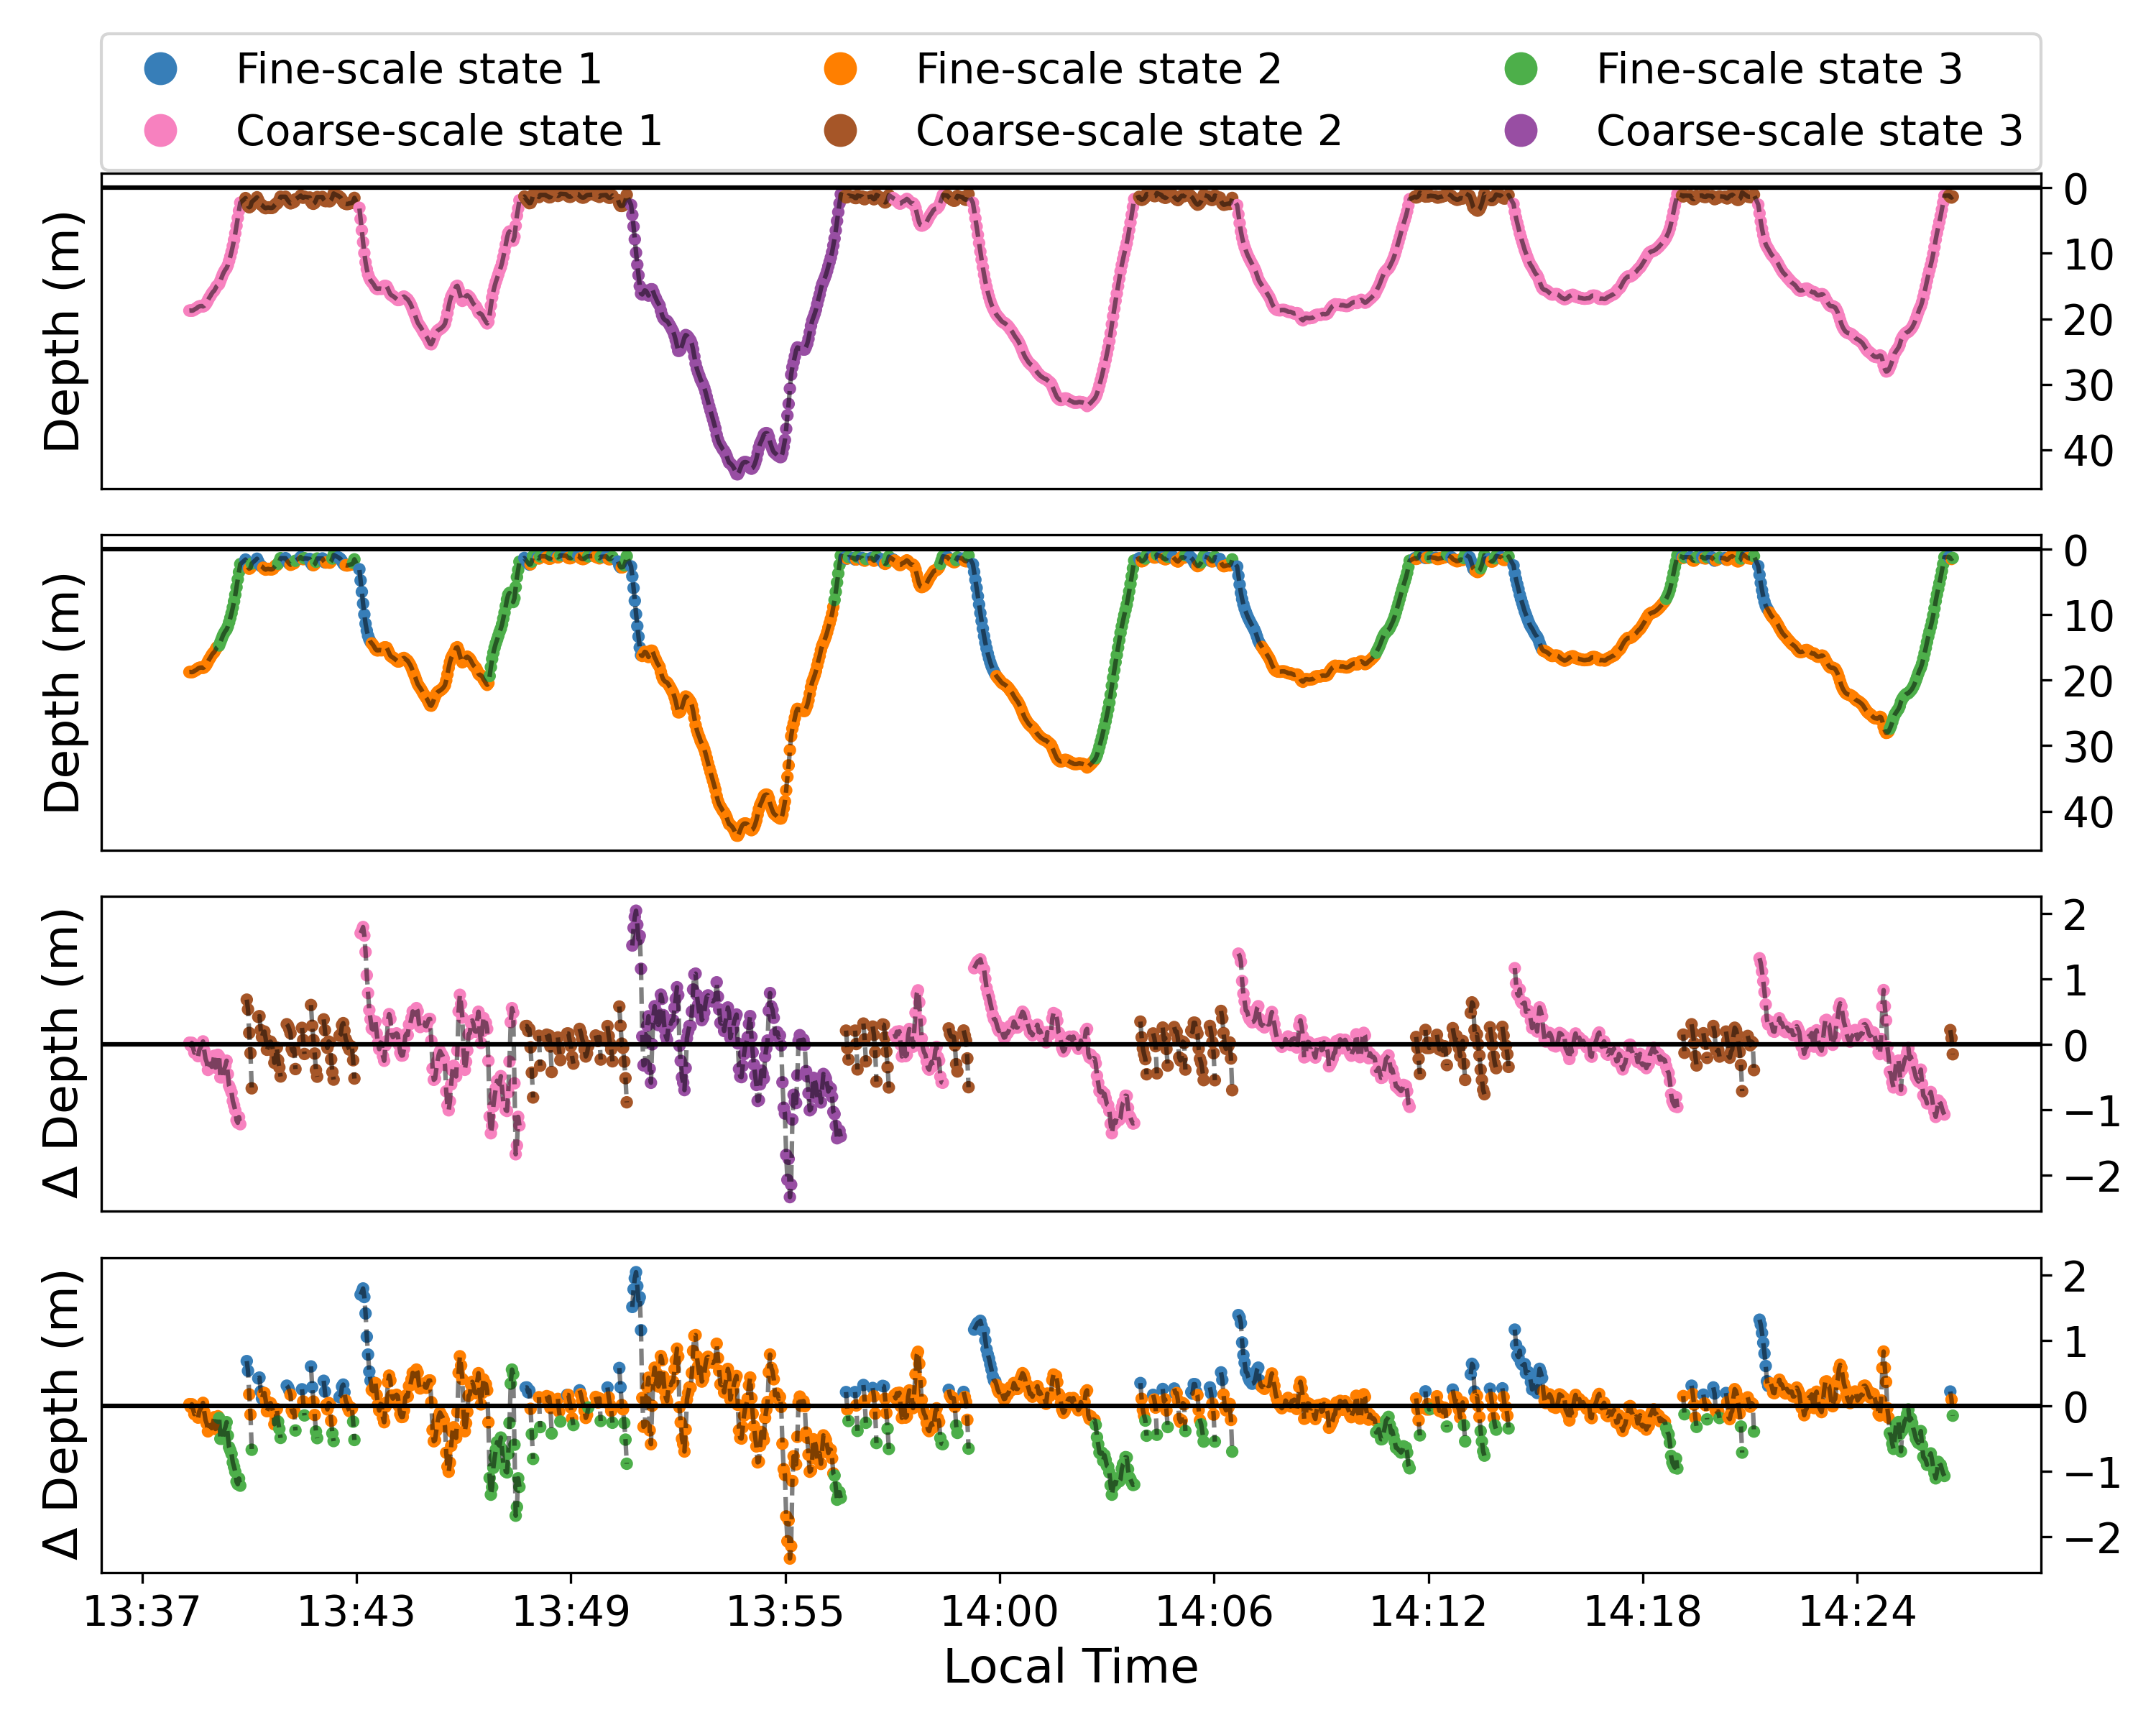
\includegraphics[width=6.5in]{../plt/decoded_dives_kw_R58_K_3_3_nWhales_8.png}
    \caption{Dive profiles and change in depth vs time for a selected hour of dive time for killer whale R58. All data is color-coded by most likely dive type (rows one and three) as well as most likely dive phase (rows two and four).}
    \label{fig:R58}
\end{figure}

\end{document}